\PassOptionsToPackage{table}{xcolor}

\documentclass[
	%parspace, % Add vertical space between paragraphs
	%noindent, % No indentation of first lines in each paragraph
	%nohyp, % No hypenation of words
	%twoside, % Double sided format
	%draft, % Quicker draft compilation without rendering images
	%final, % Set final to hide todos
]{elteiktdk}[2023/04/10]

% The minted package is also supported for source highlighting
%\usepackage[newfloat]{minted}

% Document's metadata
\title{Vízközeli hulladéklerakók megbízható detektálása multispektrális műholdfelvételek segítségével}
\date{2024}

% Author(s)' metadata
\author{Dénes Botond}
\degree{programtervező informatikus MSc}
\period{2. évfolyam}

% Superivsor(s)' metadata
\supervisor{Cserép Máté}
\affiliation{egyetemi tanársegéd}

% University's metadata
\university{Eötvös Loránd Tudományegyetem}
\faculty{Informatikai Kar}
\department{Programozáselmélet és Szoftvertechnológiai Tanszék}
\city{Budapest}
\logo{elte_cimer_szines}

% Add bibliography file
\addbibresource{elteiktdk.bib}

% The document
\begin{document}

% Set document language
\documentlang{hungarian}
%\documentlang{english}

% List of todos (not in the final document)
%\listoftodos[\todolabel]
%\cleardoublepage

% Cover and title page (mandatory)
\makecover
\cleardoublepage
\maketitle

% Table of contents (mandatory)
\tableofcontents
\cleardoublepage

% Main content
\chapter{Bevezetés}
\label{ch:intro}

\todo{szinkronizálni az absztrakttal}A hulladékszennyezés komoly problémát jelent a természet számára \cite{kibria2023PlasticWaste}. Emiatt számos szervezet mozdul abba az irányba, hogy tisztábbá tegye a bolygónkat. Egy ilyen szervezet a PET Kupa, akik folyómenti hulladékgyűjtéssel foglalkoznak elsősorban Magyarországon, de figyelmük kiterjed a szomszédos országokra is. Az egyik nagy kihívás a szemétgyűjtésben a hulladékkal szennyezett területeknek a hatékony megtalálása. Sok erőforrást igényel a hulladéklerakók megtalálása a folyók mentén, hiszen sokszor járművel kell valakinek végig haladnia egy hosszabb területen, azért, hogy felmérje, hogy hol van hulladék. A folyók árterén elhelyezett hulladékok még nagyobb problémát jelentenek, hiszen dagály idejében a hulladékot elmossa a víz és ez a folyó további szakaszaira lesz szétszórva miközben nagy károkat okoz a folyó élővilágának, illetve szennyezi a folyóvizet \cite{nyberg2023, vanEmmerik2023}. Emiatt szükségünk van olyan eszközökre, melyekkel hamar lehet detektálni a szennyezett területeket, hogy ezeket minél hatékonyabban meglehessen tisztítani. Az ELTE Térinformatikai Labor és a PET Kupa együttműködésében olyan eszközöket fejlesztünk, melyek automatikusan képesek lesznek hulladékot detektálni a folyók mentén.

A dolgozatomban bemutatok egy Random Forest modellt \cite{breiman2001}, mely a kutatólaborban már lefejlesztett modellre épül \cite{magyar2023}. A bemutatott modell javít a korábbi megoldás pontosságán, illetve nagyobb megbízhatósággal találja meg a hulladékot a folyókon és a folyók mentén. A modell eredményei integrálásra kerülnek a Tiszta Tisza webalkalmazásba\footnote{A Tiszta-Tisza webalkalmazás hivatalos weboldala a https://tisztatiszaterkep.hu/ címen található, de a dolgozatban említett fejlesztések jelenleg a https://gis.inf.elte.hu/tiszta-tisza/ oldalon érhetőek el.}, ahol több napon keresztül történő detektálás eredménye lesz összesítve és megjelenítve a felhasználók számára. Ezen felül a dolgozatban tárgyalni fogok más kutatást is, mely a hulladékdetektálás problémájával foglalkozik. Ezen kívül kiegészítem a kutatólabor meglevő szoftveres eszközeit annak érdekében, hogy a laborban zajló munka gördülékenyebb legyen.
\todo[inline,color=blue!50]{Hivatkozd meg a https://tisztatiszaterkep.hu/ oldalt, de említsd meg, hogy a prototípus egyelőre a https://gis.inf.elte.hu/tiszta-tisza/ oldalon érhető el. Ez mehet akár csak lábjegyzetbe. Botond: Rendben, lábjegyzetben megemlítettem.}

A kutatás hozzáadott terméke egy olyan adathalmaz, mely alkalmas más hulladékdetektálási modellek betanítására is. Az adathalmaz elsősorban szárazföldi romániai hulladéklerakókról készített PlanetScope műholdfelvételeket tartalmaz, melyek kézzel voltak annotálva. Az adatok georeferálva vannak, így ezeket könnyen meg lehet vizsgálni, illetve ki lehet egészíteni.

Továbbá bemutatom, hogy milyen módszerekkel próbáltam tovább javítani a modell eredményein. Ilyen módszer például a főkomponens analízis, a képnormalizálás, illetve az évszakokra bontás.

\section{A kutatólabor eddigi eredményei}

A ELTE IK Térinformatikai Kutatólaborában már betanításra került egy Random Forest modell, mely folyómenti hulladék detektálására alkalmas. Az én dolgozatomban, a kutatólabor meglevő tudására építve, továbbfejlesztem ezt a modellt, hogy kevesebb \textit{false positive}-al találja meg a szeméttel szennyezett területeket. Továbbra implementálásra került egy szerveralkalmazás, mely minden nap a Planet szervereiről letölti a legfrissebb felvételeket a vizsgált területekről, és lefuttatja ezeken a képeken az akkori modellt. Ezen felül készült egy webalkalmazás is, ami erről a szerverről letölti az eredményeket, és megjeleníti ezeket, összehasonlításra. A kutatólabor rendelkezik egy asztali alkalmazással is, mellyel hatékonyan elő lehet állítani tanító adatokat. A kutatásom elősegítéséhez ezeket az alkalmazásokat használtam, illetve bővítettem a \ref{ch:application-improvement} fejezetben leírtak szerint.

\section{Kutatási cél}
\label{ch:goals}

A cél az, hogy a kutatás során szerzett modell megbízhatóan detektáljon hulladéklerakókat általánosan folyók mentén. Ehhez a \textit{false positive} arányok minél kisebbek kell legyenek, míg a true positive arányok minél nagyobbak. Ugyanakkor nem jelent ugyanakkora problémát egy \textit{false negative}, mint egy \textit{false positive}, mivel a \textit{false positive} eredmények fölöslegesen rossz irányba küldhetik a folyómentő csapatot. 
A kutatólabor 2023-as cikkében bemutatott modell (továbbiakban meglevő modell vagy régi modell) \cite{magyar2023} egyik problémája a nagy \textit{false positive} arányok voltak. Általában a modellnek leginkább az utak, épületek okoznak problémát. Ez annak köszönhető, hogy a hulladék, a törmelék, az épületek, és a föld nagyon hasonló spektrális értékekkel rendelkeznek a használt sávokon. A modell a pusztazámori hulladéklerakóról, illetve a kiskörei víztárolóról szerzett adatokkal volt betanítva. Ezért egy jó irány több adaton betanítani a modellt, nagy figyelmet fektetve arra, hogy az adathalmaz tartalmazzon bőven utakat, épületeket, és más adatokat, amik hasonlítanak a hulladékra. 

\section{A dolgozat felépítése}
A \ref{ch:related_research}. fejezetben bemutatásra kerülnek a hulladékdetektálás témáját feldolgozó kutatások, illetve bemutatom azokat a technikai és számolási eszközöket, melyek lényeges szerepet vállalnak a kutatásomban.
A \ref{ch:training}. fejezetben részletezem a Random Forest modell betanításához előállított adatokat, a modell betanítási paramétereit, illetve megvizsgálok különböző adatfeldolgozási módszereket, ilyen például a főkomponens analízis, képnormalizálás, vízmaszkolás, azzal a céllal, hogy tovább javítsak a modell teljesítményén. A \ref{ch:verification}. fejezetben tárgyalom a modell tesztelésének és validálásának módját, illetve a tesztadatok megválasztásának módját, motivációját. A \ref{ch:impl}. fejezetben bemutatom a kutatást lényegesen előresegítő szoftveres fejlesztéseket, azt, hogy a kutatás eddigi eredményei miként vannak integrálva a Tiszta-Tisza alkalmazásba. A \ref{ch:sum}. fejezetben összefoglalom a kutatás eredményeit, és ezek alapján tárgyalom a kutatás további lehetséges haladásait. 
\cleardoublepage

\chapter{Kapcsolódó kutatások}
\label{ch:related_research}

\section{Hulladékdetektálási módszerek}

A hulladékdetektálás témája viszonylag új, és számos fejlemény történt az évek során, tekintve, hogy a légi és műholdfelvételek minősége is nőtt. Emiatt kevés olyan kutatás létezik, mely pontosan azzal a problémával foglalkozik, amivel ebben a dolgozatban foglalkoztam, de az érintőleges kutatások is olyan módszereket, ötleteket mutatnak be, melyeket érdemes megfontolni ebben a kutatásban is. Az én kutatásom a Térinformatikai kutatólabor munkájára épül \cite{magyar2023}, ahol egy Random Forest modell került betanításra, hulladékdetektálás céljából. A kutatásban PlanetScope és Sentinel-2 műholdfelvételeket használtak. Ez a cikk rakta le az alapjait az én kutatásomnak is, melyben ezeken az eredményeken javítok. A cikkben további lehetséges munkaként említésre kerül a modell több adattal való tanítása, illetve a képfeldolgozás gyorsítása. A dolgozatom mindkét feladattal foglalkozik, A dolgozatomban csak a PlanetScope felvételek kerülnek felhasználásra, mivel a magasabb felbontású felvételek könnyebben lehetővé teszik a tanítóadatok előállítását, hiszen jobban lehet látni a hulladéklerakókat rajtuk.

\cite{sakti2023}-ben Sentinel-2 műholdfelvételeken tanítottak be egy Random Forest modell-t azzal a céllal, hogy egy indonéziai folyóban detektáljanak hulladékot. A cikkben bevezetik az "Adjusted Plastic Index"-et, mellyel a vegetáció, föld és épületek közötti zajt csökkentik. Ennek az indexnek a kiszámításához a Sentinel-2 műhold piros, közeli infravörös (NIR), illetve rövid hullámhosszú közeli infravörös (SWIR) sávokat használták fel. Validációnak Pleiades műholdképeket és drónfelvételeket klasszifikáltak Mahalanobis távolság gépi tanulási módszerrel (\ref{fig:sakti} ábra). A módszer növényzeten és vízen rendre 88\%, illetve 85\% pontosságot ért el és épületeken, törmeléken és földön rendre 62\%, 53\%, illetve 21\% pontossággal tudta a hulladékot detektálni. A cikk szerint az utóbbi három adattípuson azért visszafogottabbak az arányok, mert a spektrális értékei az épületeknek, a földnek és a törmeléknek nagyon hasonlítanak.

\begin{figure}[H]
	\centering
	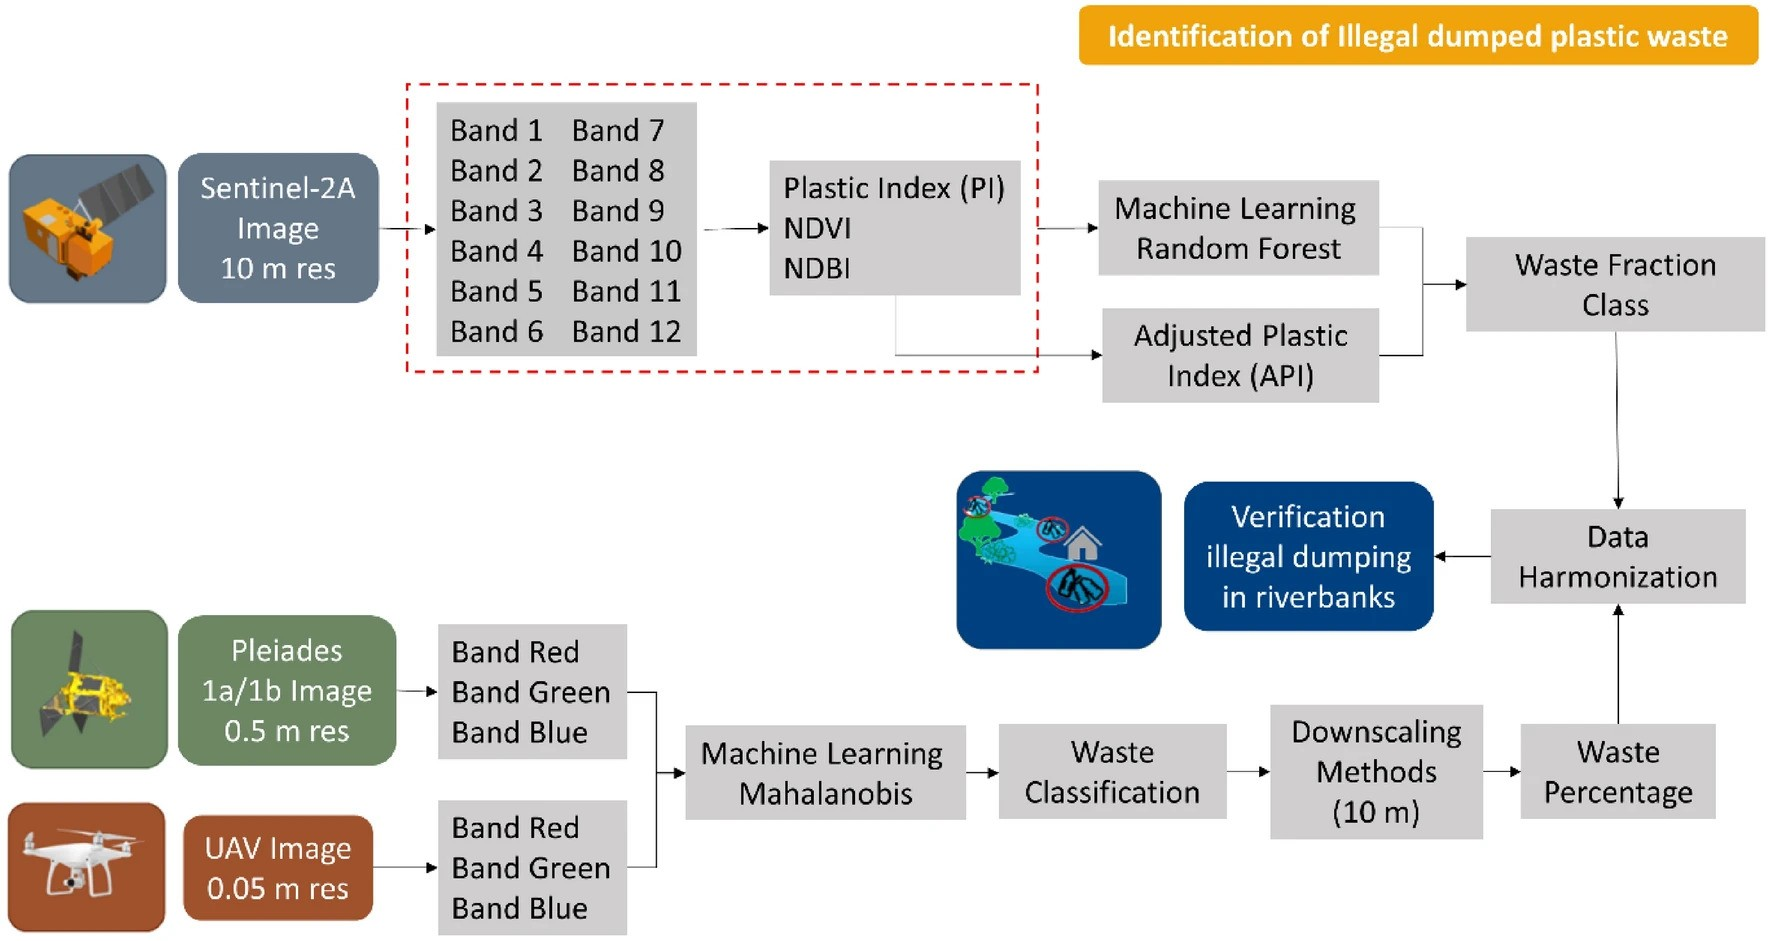
\includegraphics[width=0.6\textwidth,frame]{sakti}
	\caption{Hulladékdetektálás "Adjusted Plastic Index", Random Forest és Mahalanobis távolság segítségével \cite{sakti2023}}
    \label{fig:sakti}
\end{figure}


\cite{goncalves2022}-ben Spectral Angle Mapping módszert alkalmaztak multispektrális drónfelvételeken, egy Portugál tengerparton. A célja a kutatásnak az volt, hogy a tengerparton kimosott hulladékot detektálják és klasszifikálják. A módszer alkalmazásához referencia értékeket állítottak elő azzal, hogy elhelyeztek különböző anyagokból álló hulladékot a homokba, és ezekről drónfelvételt készítettek (\ref{fig:goncalves} ábra). Ezzel a módszerrel képesek voltak detektálni és klasszifikálni nem csak homok fölött található hulladékot, hanem a homokban félig elásott hulladékot is. A 472 kézzel előállított tesztadatból volt a 268 True Positive (57\% összesen), 96 volt a False Positive és 204 volt a False Negative.

\begin{figure}[H]
	\centering
	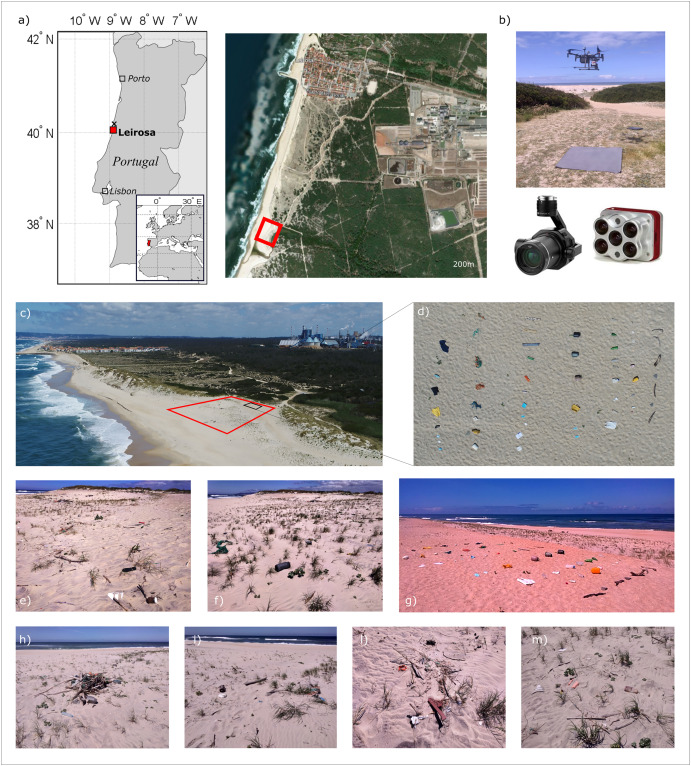
\includegraphics[width=0.6\textwidth,frame]{goncalves}
	\caption{Spectral angle mapping referencia adatainak előállítása \cite{goncalves2022}}
    \label{fig:goncalves}
\end{figure}

\cite{lanorte2017}-ben mezőgazdasági hulladékdetektálásra használtak egy Support Vector Machine modellt, Landsat 8 műholdfelvételeken. A szenzor Kék, Zöld, Piros, NIR, SWIR 1, SWIR 2 és CIRRUS sávját használták a tanítóadatok és tesztadatok előállítására. Ezután véletlenszerűen szétválasztották az adatokat tanítóadatokra és tesztadatokra. A következő osztályokra bontották az adatokat: Hálók, műanyag takarók, föld, növényzet, gyümölcsöskert, olajfás kert, város, fa, fás föld. A modell a tesztadatokat összességében 94\%-os pontossággal tudta klasszifikálni, ahol a legrosszabb arányokat az olajfás kert érte el 77.78\%-os pontossággal.

\cite{zeng2019}-ben a hiperspektrális adatokon tanítottak be egy felügyelt és egy felügyeletlen gépi tanulási módszert. A működési elv az, hogy a felügyelt módszerrel klasszifikálják a hulladékkal szennyezett területeket, míg a felügyeletlen módszerrel megbecsülik a hulladékkal szennyezett terület kerületét (\ref{fig:zeng} ábra). Ők 99.89\%-os kappa együtthatóval tudtak hulladékot detektálni \todo{Átnézni mégegyszer a cikket és átvizsgálni az adatok helyességét}.

\begin{figure}[H]
	\centering
	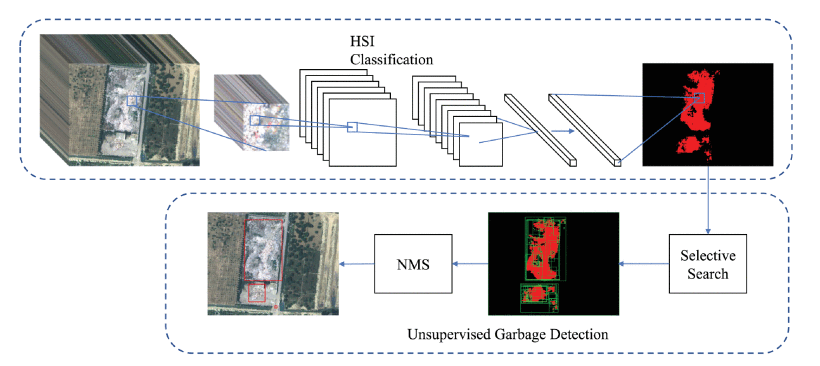
\includegraphics[width=0.6\textwidth,frame]{zeng}
	\caption{Az MSCNN működési elve \cite{zeng2019}}
    \label{fig:zeng}
\end{figure}

\cite{sun2023}-ben megvizsgálják azt, hogy mennyivel lesz hatékonyabb a hulladékkezelés a manuális vizsgálat helyett, ha egy mély tanulás alapú hulladékdetektálási módszert használnak a hulladékkezeléshez magas (0.3m-1m per pixel) felbontású műholdfelvételeken. Négy osztályba bontják a hulladékot: háztartási hulladék, mezőgazdasági hulladék, építkezési hulladék, lefedett hulladék. A modell képes 98\%-át detektálni a hulladéklerakóknak a teszthalmazban, illetve az automata detektálás segítségével több, mint 96.8\%-al csökkentették azt az időt, ami a hulladékdetektálás vizsgálatára kellett. Ráadásul a modell könnyen telepíthető egy laptopra, és 30 másodperc alatt le tudja futtatni a modellt a 162 négyzetkilóméteres tesztadathalmazon. A betanításhoz mindössze 2500 hulladéklerakót annotáltak világszerte kézzel 4800 négyzetkilóméteren keresztül. A \ref{fig:bca-net-working} ábrából látható a módszer működési elve: a modell a spektrális értékek mellett a hulladéklerakó alakját is figyelembe veszi. A megfelelő magabiztosságú területek hulladéklerakóként lesznek címkézve. A modellt betanító és validáló kód, illetve az adathalmaz, mellyel az eredmények reprodukálhatóak elérhetőek a cikkből.

\begin{figure}[H]
	\centering
	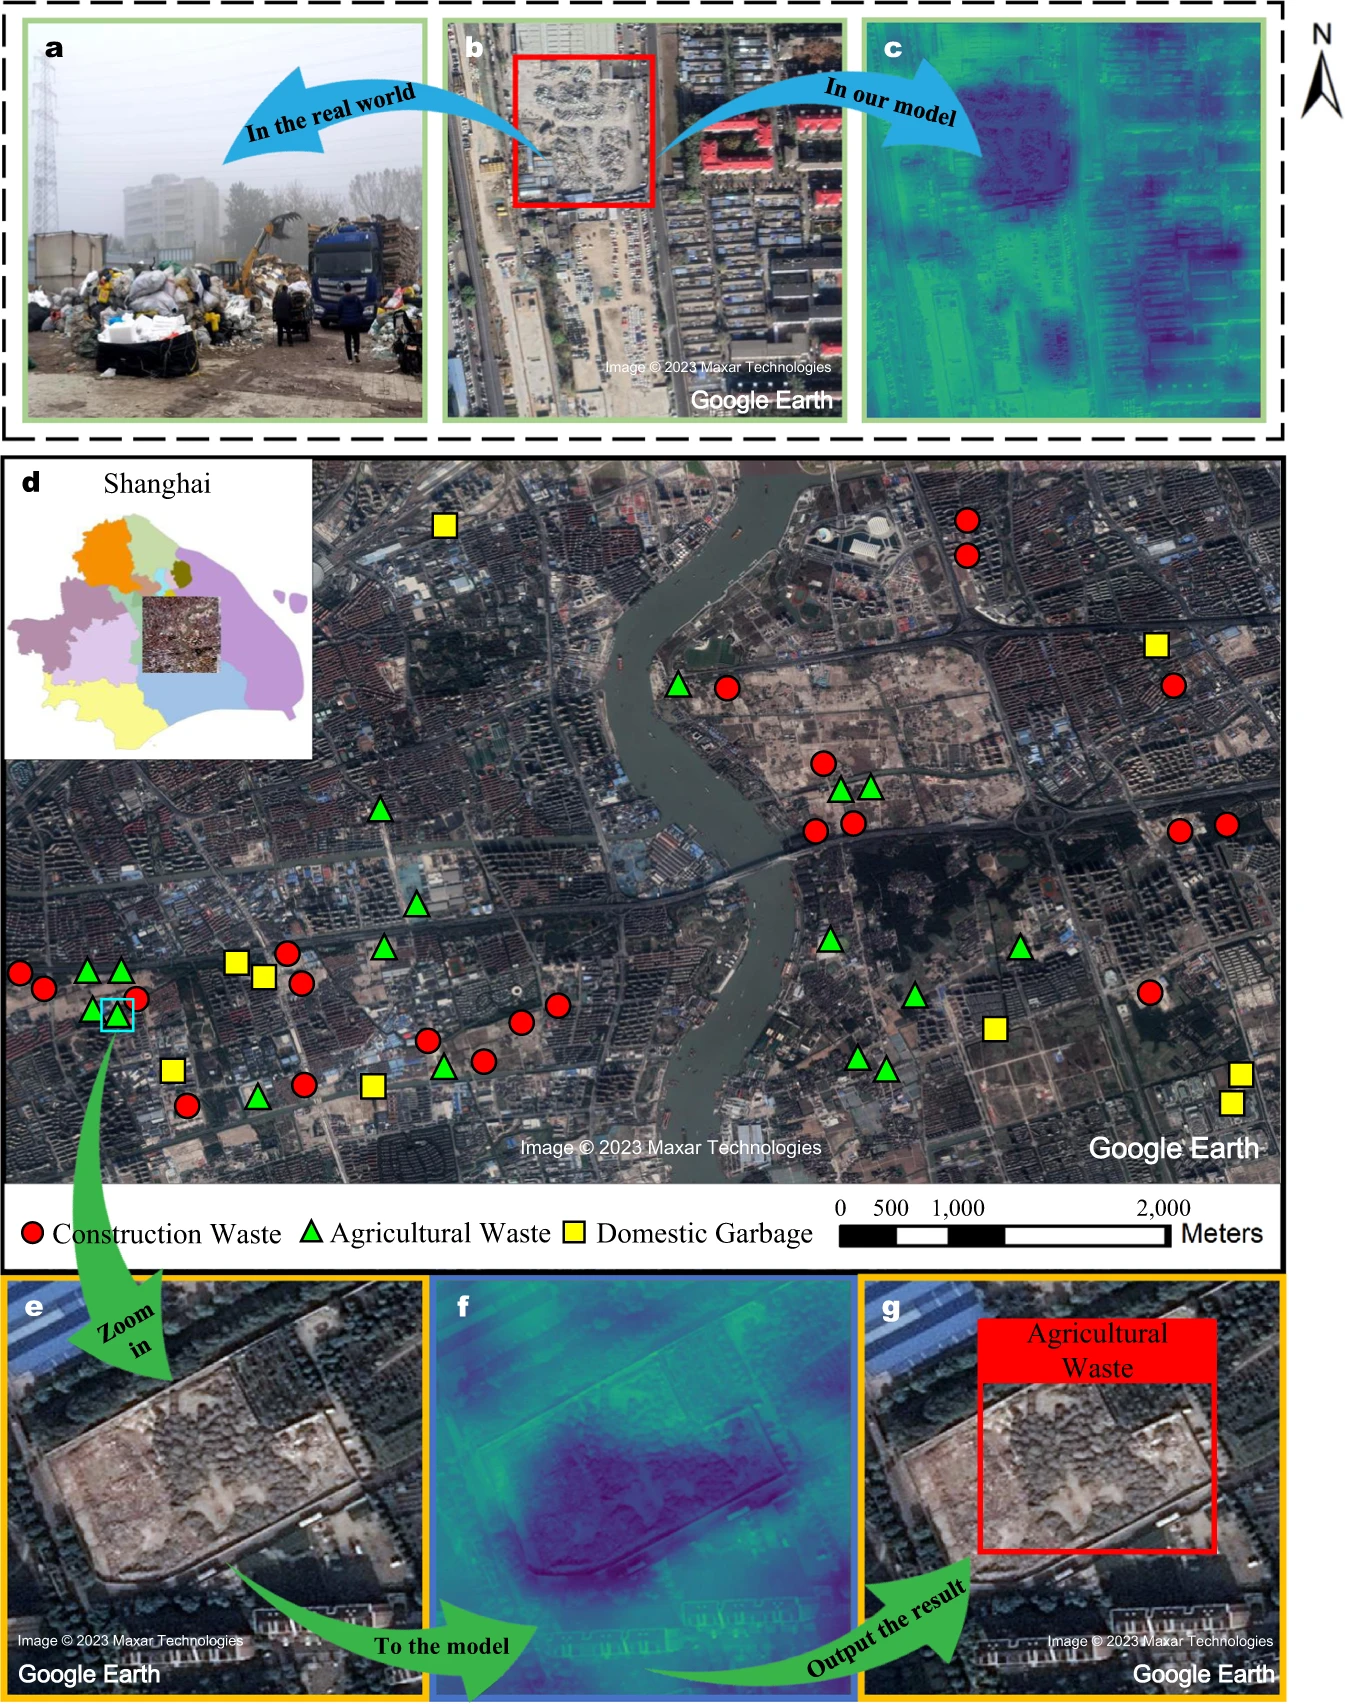
\includegraphics[width=0.6\textwidth,frame]{bca-net}
	\caption{Az BCA-Net működési elve \cite{sun2023}}
    \label{fig:bca-net-working}
\end{figure}

\cite{Torres2021} egy konvolúciós neuronhálót használ, mely 94.5\%-os átlagos pontossággal és 88.2\%-os F-Score-al rendelkezik. A tanító adathalmaz 3000 ortofotóból áll, melyek 20cm per pixel felbontással rendelkeznek és a vörös, kék és zöld tartományokat tartalmazzák. A felvételeket szakértők annotálták, kézzel. A modell a ResNet50 \cite{ResNet2016} hálóra épül és a Feature Pyramid Network \cite{FPN2017} architektúrával van kiegészítve. A modell figyelembe veszi a hulladéklerakó alakját és kontextusát, mely segít a hulladékdetektálás pontosságának a növelésében.

\cite{Taggio2022} tengeri hulladékdetektálással foglalkozott Görögország területén levő tengerpartokon: egy felügyelt (Light Gradient Boosting Model) és egy felügyeletlen (K-Means) gépi tanulási algoritmust alkalmaztak PRISMA hiperspektrális műholdfelvételeken, mellyel átlagosan 96\%-os pontosságot értek el. A tanítóadatokat kontrollált környezetben állították elő (\ref{fig:marine-data-controlled}): különböző környezeteket szimutálva vízre helyeztek különböző anyagokból álló hulladékokat, melyekről műholdfelvételek készültek. Ennek köszönhetően pontosan elő tudták állítani a tanítóadatokat \todo{átfogalmazni, mégegyszer elolvasni a cikket}.

\begin{figure}[H]
	\centering
	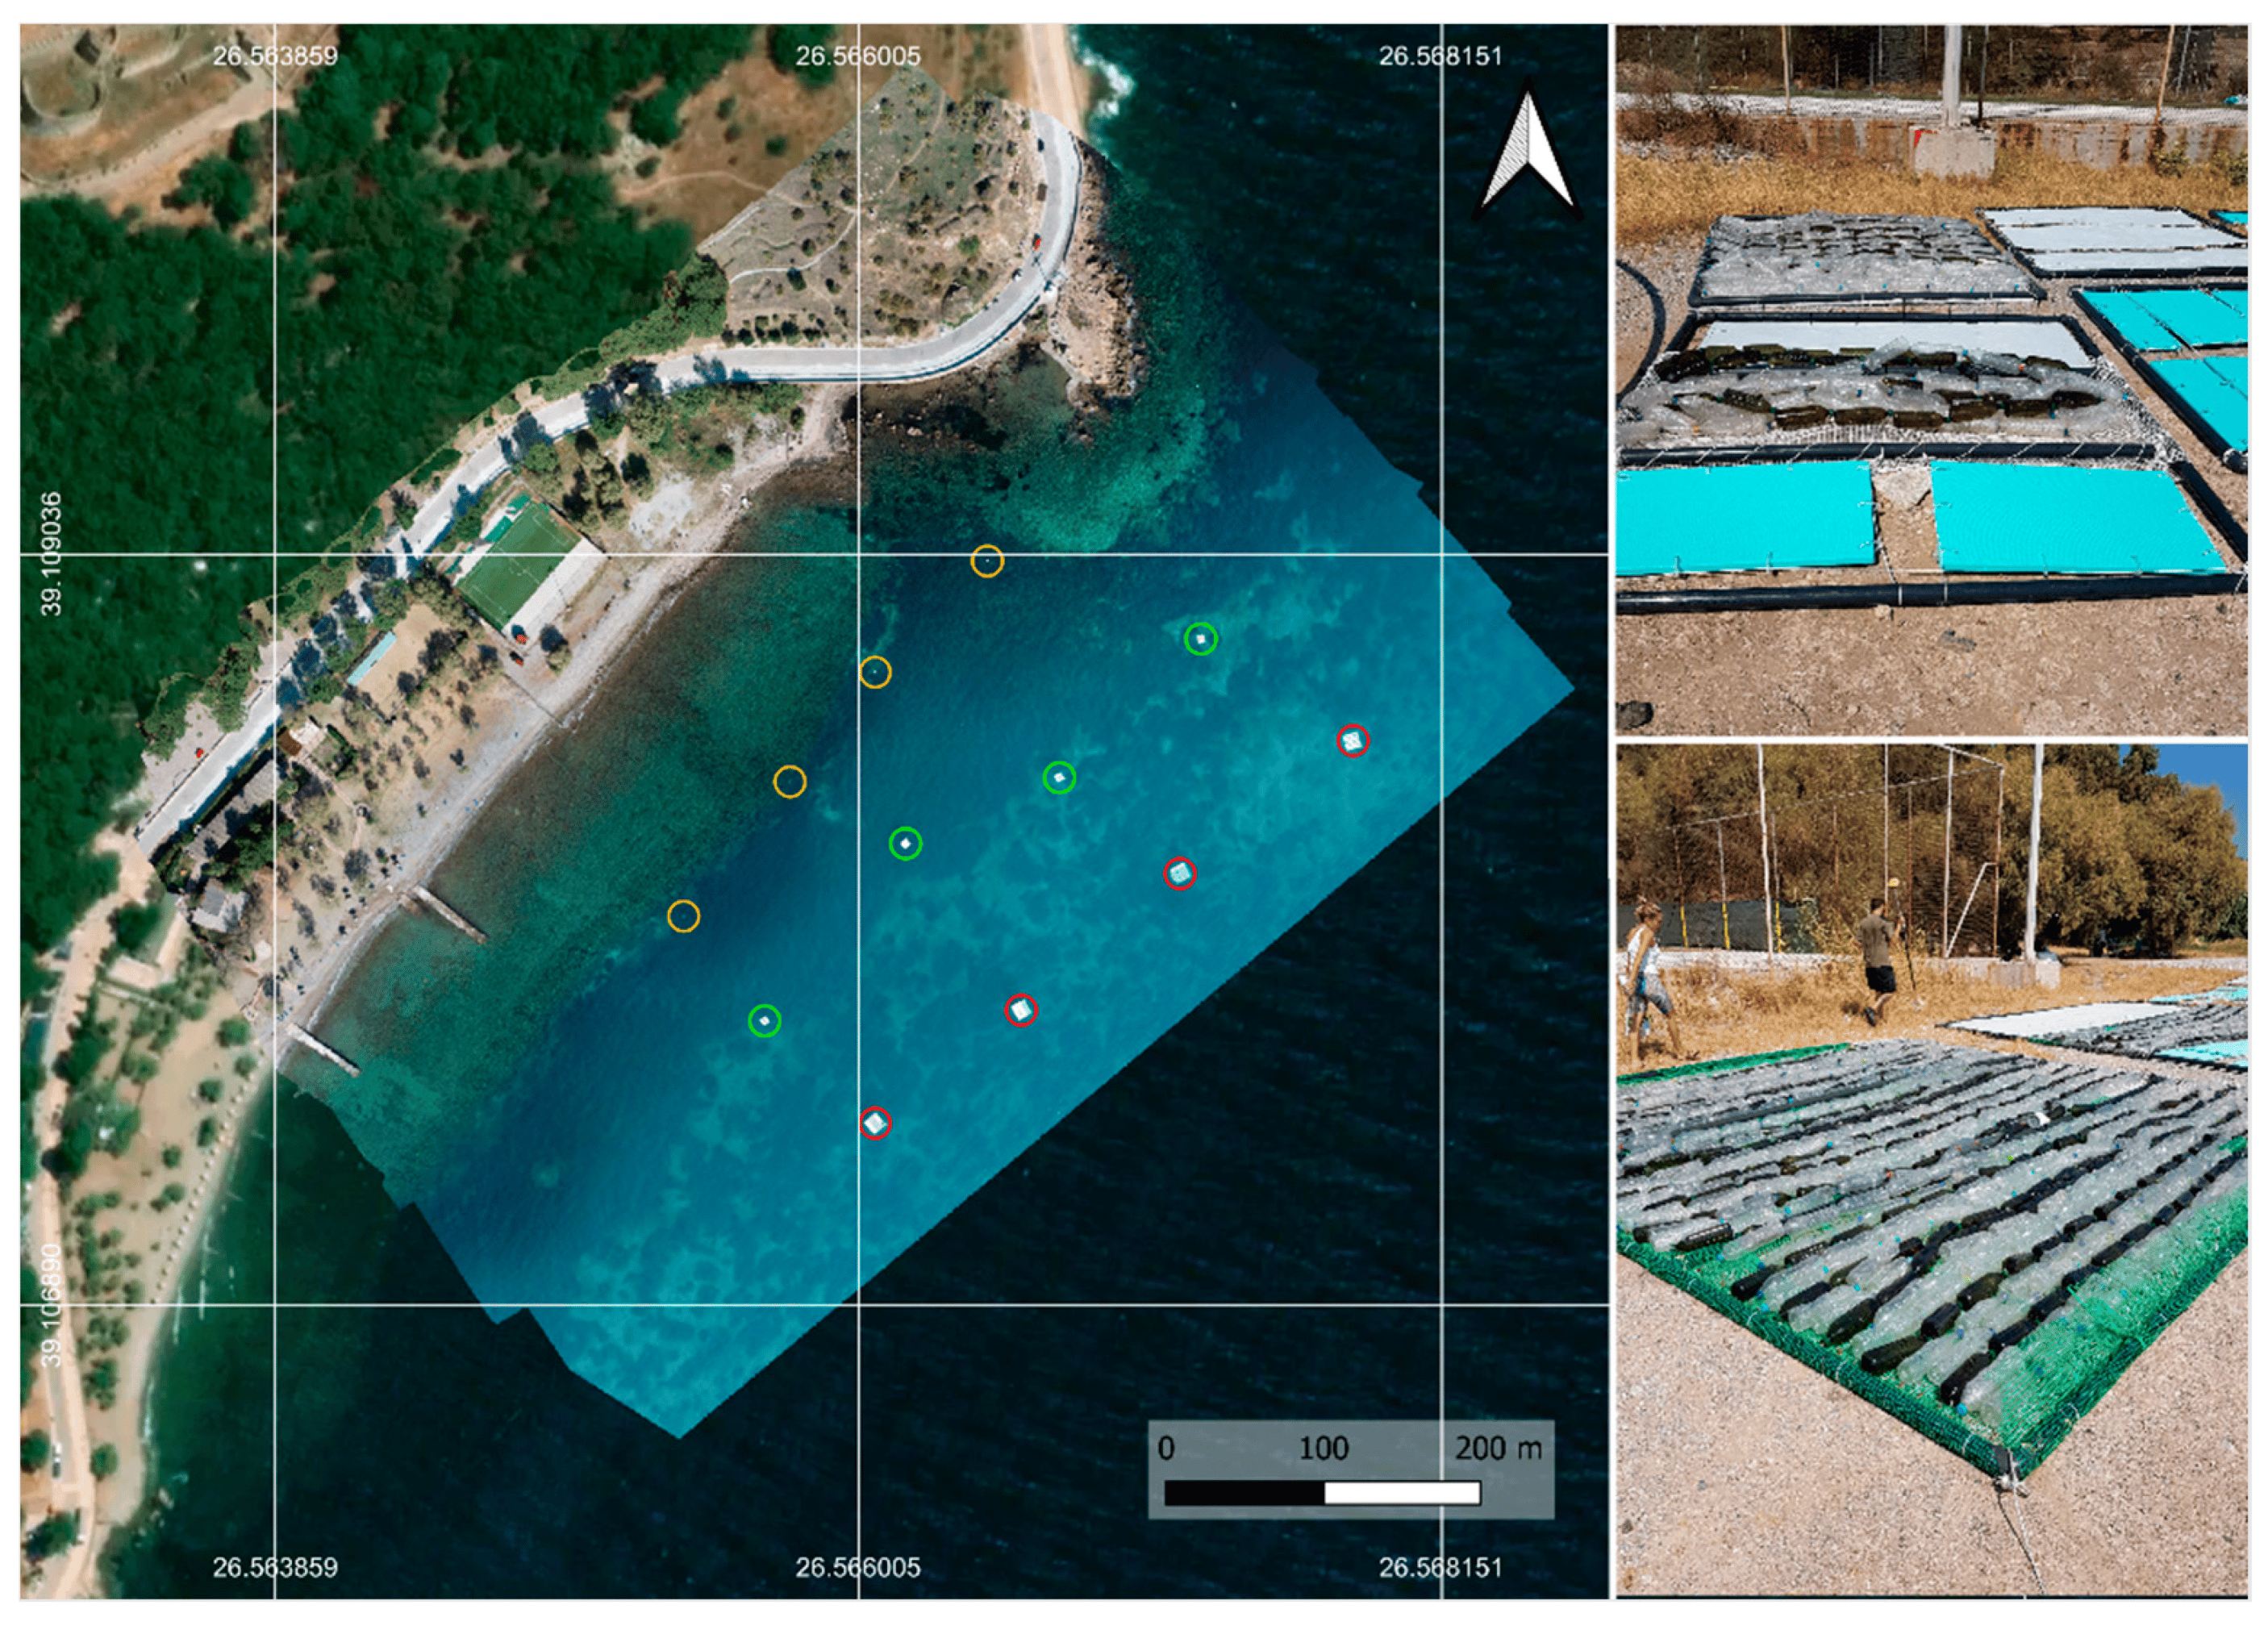
\includegraphics[width=0.6\textwidth,frame]{marine-data-controlled}
	\caption{A tengeri hulladékdetektáláshoz való tanítóadatok előállítása \cite{Taggio2022}}
    \label{fig:marine-data-controlled}
\end{figure}

\cite{Wolf2020}-ban tengerparti hulladékdetektálással foglalkoztak, úgy úszó hulladékkal, mint partra kimosott hulladékkal. A kutatásban bemutatnak egy APLASTIC-Q konvolúciós neuronhálót, mely 5 pixel per cm felbontással rendelkező felvételeket klasszifikált Kambodzsa területén . A modell két fő komponensből állt: egy műanyag-hulladék detektálóból (PLD-CNN) és egy műanyag-hulladék osztályozóból (PLQ-CNN). A PLD-CNN megkülönböztette a vizet, homokot, növényzetet és műanyag alapú hulladékot 83\% átlagos pontossággal, illetve megállapította, hogy az adott terület mennyire hulladékos. PLQ-CNN megkülönböztette a különböző hulladék típusokat átlagosan 71\%-os pontossággal: ilyenek például az üvegpalackok, cipők, textil anyagok stb. A PLD-CNN betanításához 5515 darab 100 × 100 × 3 pixeles csempét használtak, míg a PLQ-CNN betanításához 4828 darab 50 × 50 × 3 pixeles csempékre vágták a felvételeket. 

\cite{Goncalves2020}-ban gépi tanulást, geomorfológiát, fotogammetriát és hidrodinamikai modellezést kombinálnak össze azzal a céllal, hogy homokos partok környékén, illetve homokdombokon detektáljanak hulladékot drónfelvételek segítségével (\ref{fig:goncalves2020-method} ábra \todo{jobb ábrát keresni}). A geomorfológiai vizsgálat segítségével megtudták különböztetni a partokat és a homokdombokat, mellyel optimizálni tudták a hulladékdetektálást. A gépi tanulási modell egy Random Forest volt, mellyel a homokban található hulladékot detektálták. A hidrodinamikai számolások segítségével meg lehetett becsülni, hogy hol kerülnek a hulladékok kimosásra, illetve a parton található hulladékok mennyit fognak ott maradni. Összességében ezzel a módszerrel a hulladékdetektálás 75\%-os F-Score-al sikerült.

\begin{figure}[H]
	\centering
	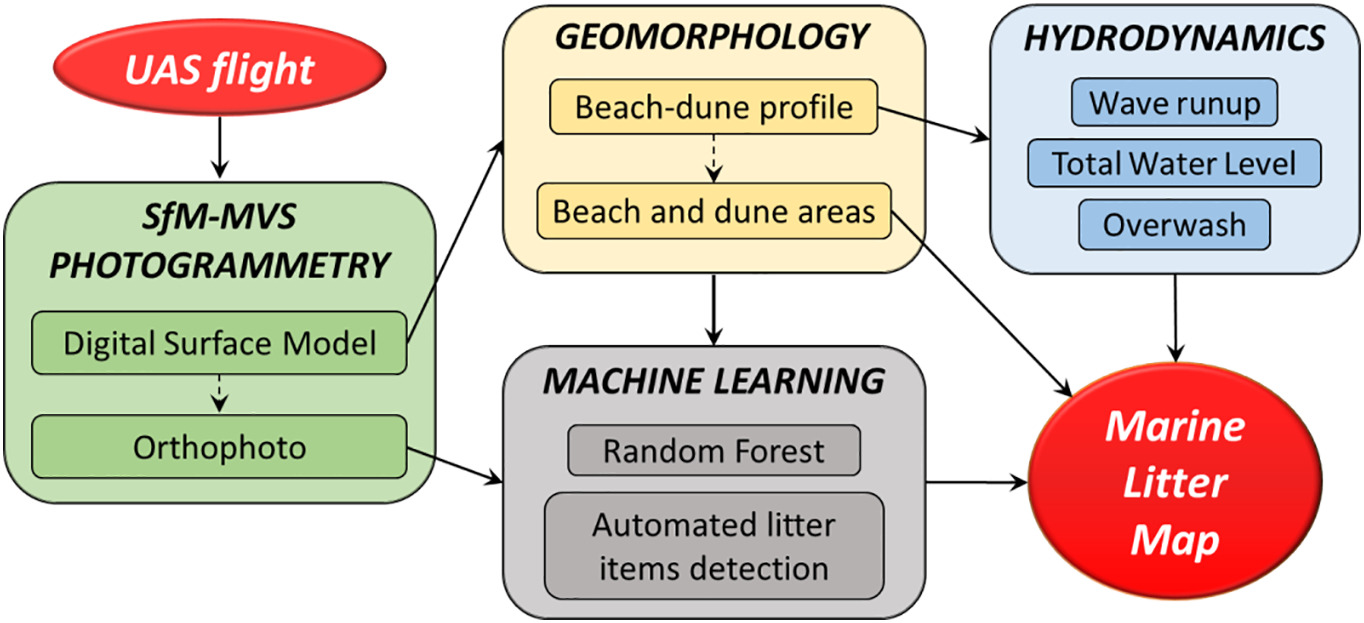
\includegraphics[width=0.6\textwidth,frame]{goncalves2020}
	\caption{A gépi tanulás, geomorfológia, fotogammetria és hidrodinamikai modellezés használása hulladékdetektálásra \cite{Goncalves2020}}
    \label{fig:goncalves2020-method}
\end{figure}



\section{Döntési fa}
\label{ch:decision-tree}

A döntési fák általános célú predikcióra és osztályozásra használt eszközök \cite{deville2013}. Az előnyeik közé tartozik az, hogy tekintve az egyszerű struktúrájukat, könnyen értelmezhetőek és rugalmasak. A \ref{fig:decision-tree} ábrából látható a döntési fa működési elve.

\begin{figure}[H]
	\centering
	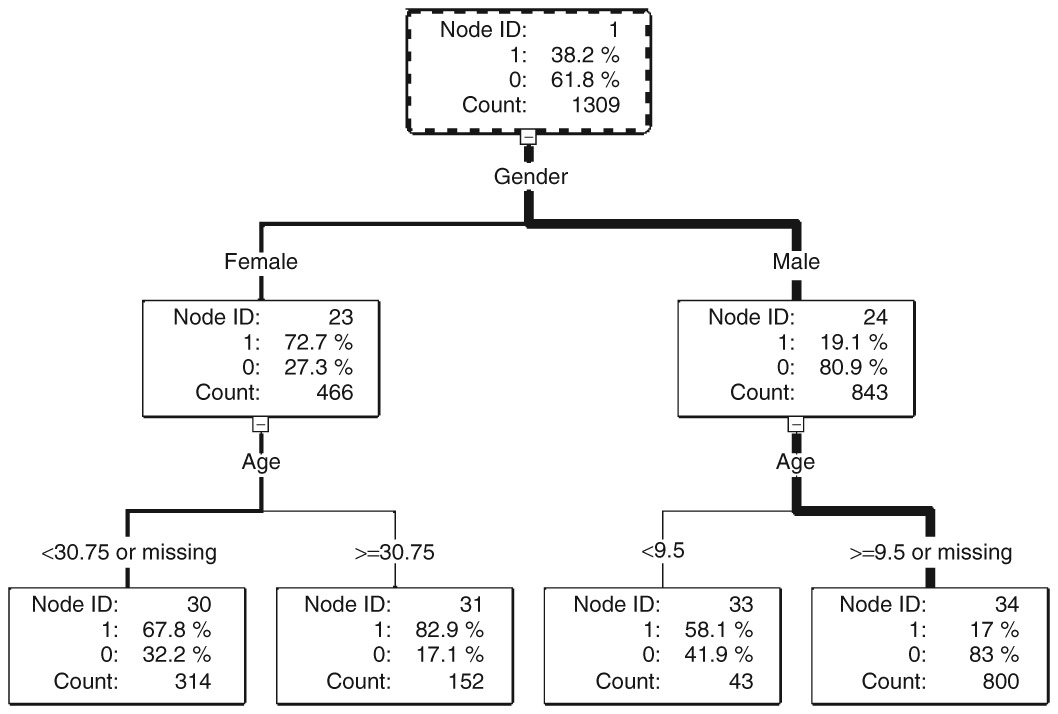
\includegraphics[width=0.6\textwidth,frame]{decision-tree}
	\caption{A döntési fa működési elve elve \cite{deville2013}}
    \label{fig:decision-tree}
\end{figure}

A \ref{fig:decision-tree} ábrán látható döntési fa a Titanic utasairól készített túlélési kutatás adatai alapján épült \cite{Harrell2013}. A fa csúcsain található 1-es címke képviseli a túlélők arányát, míg a 0-ás címke az elhunytak arányát. Mivel a 0 és 1 osztályok közül választhat a döntési fa, ezért ez egy osztályozó döntési fa. Ezen felül a csúcsban el van tárolva az is, hogy hány mérést tartalmaz. A gyökércsúcs tartalmazza az összes mérést. Ahhoz, hogy leágazzunk egy csúcsból, meg kell határoznunk a közvetlen gyerekcsúcsok "bemeneteit": ezek olyan mezők az adathalmazban, melyek a legjobban leírják a változékonyságát az adatoknak az adott szinten. A legalkalmasabb bemenetek meghatározása egy nyitott kutatási téma. Ebben a példában a gyökércsúcs közvetlen gyerekeinek a bemenete az utas neme. A következő szint bemenete pedig az utas kora. Így például a következő információkat olvashatjuk le a döntési fáról: a 30.75 év fölötti nőknek volt a legnagyobb túlélési esélyük, míg a 9.5 fölötti vagy ismeretlen életkorral rendelkező férfiaknak volt a legkisebb túlélési esélyük. Így tehát ha meg szeretnénk állapítani, hogy mennyi lett volna a túlélési esélye egy 35 éves férfinek, akkor látnánk azt a döntési fa alapján, hogy ez 17\% lenne.

\section{Random Forest}

A \ref{ch:decision-tree} fejezetben tárgyalt döntési fa egyik hátránya az, hogy hajlamos a túltanulásra. A Random Forest egy felügyelt gépi tanulási módszer, mely magas pontossággal tud rátanulni a tanítóadatokra (túltanulás nélkül), és jól kezeli a zajt \cite{breiman2001}. A módszer több, véletlenszerűen paraméterezett döntési fa felépítéséből kapta a nevét: miután felépítettük ezt a "döntési fa erdőt", az adatokat úgy lehet osztályozni, hogy egy többségi szavazást hajtunk végre az összes fa eredménye szerint (\ref{fig:random-forest} ábra). Ennek a megközelítésnek köszönhetően az egyes túltanult döntési fák kiegyenlítik egymást, így a teljes erdő nem lesz túltanítva. A fák felépítéséhez több stratégia létezik, és ezen stratégiák alapján lehet finomhangolni a modell pontosságát és méretét. Az utóbbit fontos szem előtt tartani, tekintve arra, hogy elég sok tanítóadat esetén a modell mérete lényegesen megnőhet helyes paraméterezés hiányában. Az ilyen paraméterek például a fák maximum mélysége, a fáknak átadott részadathalmaz dimenziói, egy csúcs kettéválasztásának a kritériumjai, a tanítóadatok súlyai stb. A kutatásomban ezt a modellt tanítom be, illetve paraméterezem azzal a céllal, hogy megbízható klasszifikációt tudjon biztosítani. A modell minden képkockát osztályozni fog, így a bemeneti adatok az adott terület spektrális sávjai, illetve indexei. 

\begin{figure}[H]
	\centering
	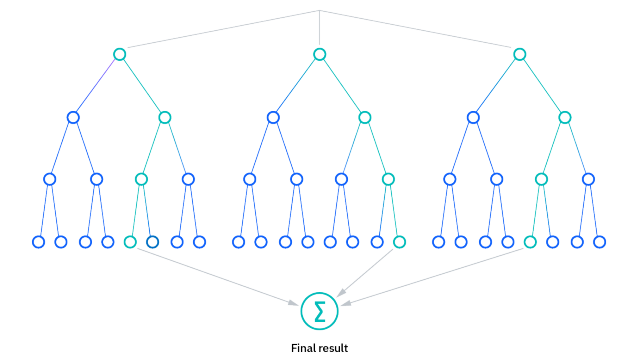
\includegraphics[width=0.5\textwidth,frame]{random-forest}
	\caption{A Random Forest működési elve \cite{IBM2024}}
    \label{fig:random-forest}
\end{figure}

\section{PlanetScope}

A Planet Labs rendszeresen műholdakat küld az űrbe azzal a céllal, hogy minden nap készüljön műholdfelvétel a Földről \cite{planetgoal2024}. A projekt jelenlegi állapotában már ott tartanak, hogy majdnem napi szintű felvételeket készítenek a Föld felszínéről több, mint 430 Dove és SuperDove műhold segítségével \cite{planetmissions2024}. A legújabb műholdcsaládjuk a SuperDove műholdakból áll. Ezek a műholdak a PSB.SD nevű műszert használják felvételek készítésére. A műszer a 47 megapixeles "PSBlue" szenzort használja.  Ezekkel a műholdakkal 2020. március közepe óta készítenek felvételeket, melyek a vörös (red), zöld (green), kék (blue), közeli infravörös (near infrared vagy NIR), illetve az úgynevezett "red edge", "green I", "coastal blue", és sárga (yellow) sávokat is tartalmazzák. Egy csempe körülbelül 32.5 x 19.6 $ km^2 $ területet fed le \cite{planetsensors2024}, körülbelül 3 méter per pixel felbontással. A \ref{tab:planet-wavelengths} táblázatból látható, hogy a PSB.SD műszer egyes sávjai milyen hullámhosszal rendelkeznek. A hullámhossz mellett jelenített "fwhm" a "Full width at half maximum" értéknek a rövidítése.

\begin{table}[H]
	\centering
	\begin{tabular}{ | p{0.2\textwidth} | p{0.2\textwidth} | p{0.2\textwidth} | }
		\hline
		\textbf{Sáv azonosító} & \textbf{Sáv neve} & \textbf{Hullámhossz (fwhm)} \\
		\hline \hline
		1 & Coastal Blue & 443 (20) \\
		\hline
		2 & Blue & 490 (50) \\
		\hline
		3 & Green I & 531 (36) \\
		\hline
        4 & Green & 565 (36) \\
		\hline
		5 & Yellow & 610 (20) \\
		\hline
		6 & Red & 665 (31) \\
		\hline
		7 & Red Edge & 705 (15) \\
		\hline
        8 & NIR & 865 (40) \\
		\hline
	\end{tabular}
	\caption{A PSB.SD műszer hullámhosszai \cite{planetsensors2024}}
	\label{tab:planet-wavelengths}
\end{table}


\cleardoublepage

\chapter{Betanítás}
\label{ch:training}

\section{Tanítóadatok}

A betanításhoz 29 romániai hulladéklerakó és közvetlen környezete került a tanítóadatok közé, illetve a Kiskörei víztároló is. A víztároló már vizsgálva volt \cite{magyar2023}-ban, és alkalmas úszó hulladéksziget detektálására, tekintve arra, hogy a felgyült faágak között nagy koncentrációban jelenik meg műanyag-alapú hulladék. A \ref{fig:kiskore-waste} ábrán látható, hogy miként gyűl össze a hulladék a víztárolónál. A romániai hulladéklerakókat egy helyi weboldalon lehet megtalálni, a hozzájuk tartozó koordinátákkal együtt \cite{wasteromania2019}. Az ott bemutatott 46 hulladéklerakó közül 29 volt alkalmas tanításra: sok hulladéklerakó be lett tömve, vagy föld alatt működik. Minden hulladéklerakóhoz letöltöttem egy-egy nyári+tavaszi, téli és őszi multispektrális műholdképet, melyeket kézzel annotáltam. A nyári és tavaszi képeket azért vontam egybe, mivel ezek hulladékdetektálás szempontjából hasonló adatokat eredményeztek. A tanítóadatok pixelenként vannak előállítva, így a végső adathalmaz 27 millió tanítóadatból (pixelből) áll. Minden pixelhez hozzá van rendelve a vörös, kék, zöld, közeli infravörös sáv, illetve a "PI", "NDWI", "NDVI", "RNDVI", "SR" indexek. Ezen felül minden pixel címkézve van a \ref{tab:waste-detection-labels} táblázatban leírtak szerint. Nagyon fontos, hogy minél pontosabban meg lehessen állapítani, hogy a hulladéklerakókon mely területeken található hulladék, hiszen sok hulladéklerakón törmeléket is tárolnak, ezt általában egy külön területen. Emiatt a tanítóadatokat a következő módszerrel állítottam elő: Megvizsgáltam Google Maps segítségével \cite{googlemaps2024}, hogy az adott hulladéklerakónál hol tárolnak törmeléket és hol tárolnak műanyag alapú hulladékot. A Google Maps légi felvételei elég magas felbontással rendelkeznek ahhoz, hogy általában szemmel meglehessen különböztetni a műanyag alapú hulladékot a törmeléktől. A \ref{fig:waste-vs-debris} ábrából látható, hogy míg a törmelék inkább fehér színt tartalmaz, addig a műanyag alapú hulladék picit vörösebb, tekintve arra, hogy a műanyag sokszor színezve van. Emellett, a hulladéklerakókat nagyon konzervatívan jelöltem ki: csak akkor jelöltem be egy területet, mint hulladékos terület, ha a felvételből egyértelmű volt, hogy az adott terület műanyag alapú hulladékkal szennyezett. Természetesen, helyi terepvizsgálattal, illetve magasabb felbontású felvételek készítésével pontosabb adatokat lehetne előállítani. 

\begin{figure}[H]
	\centering
	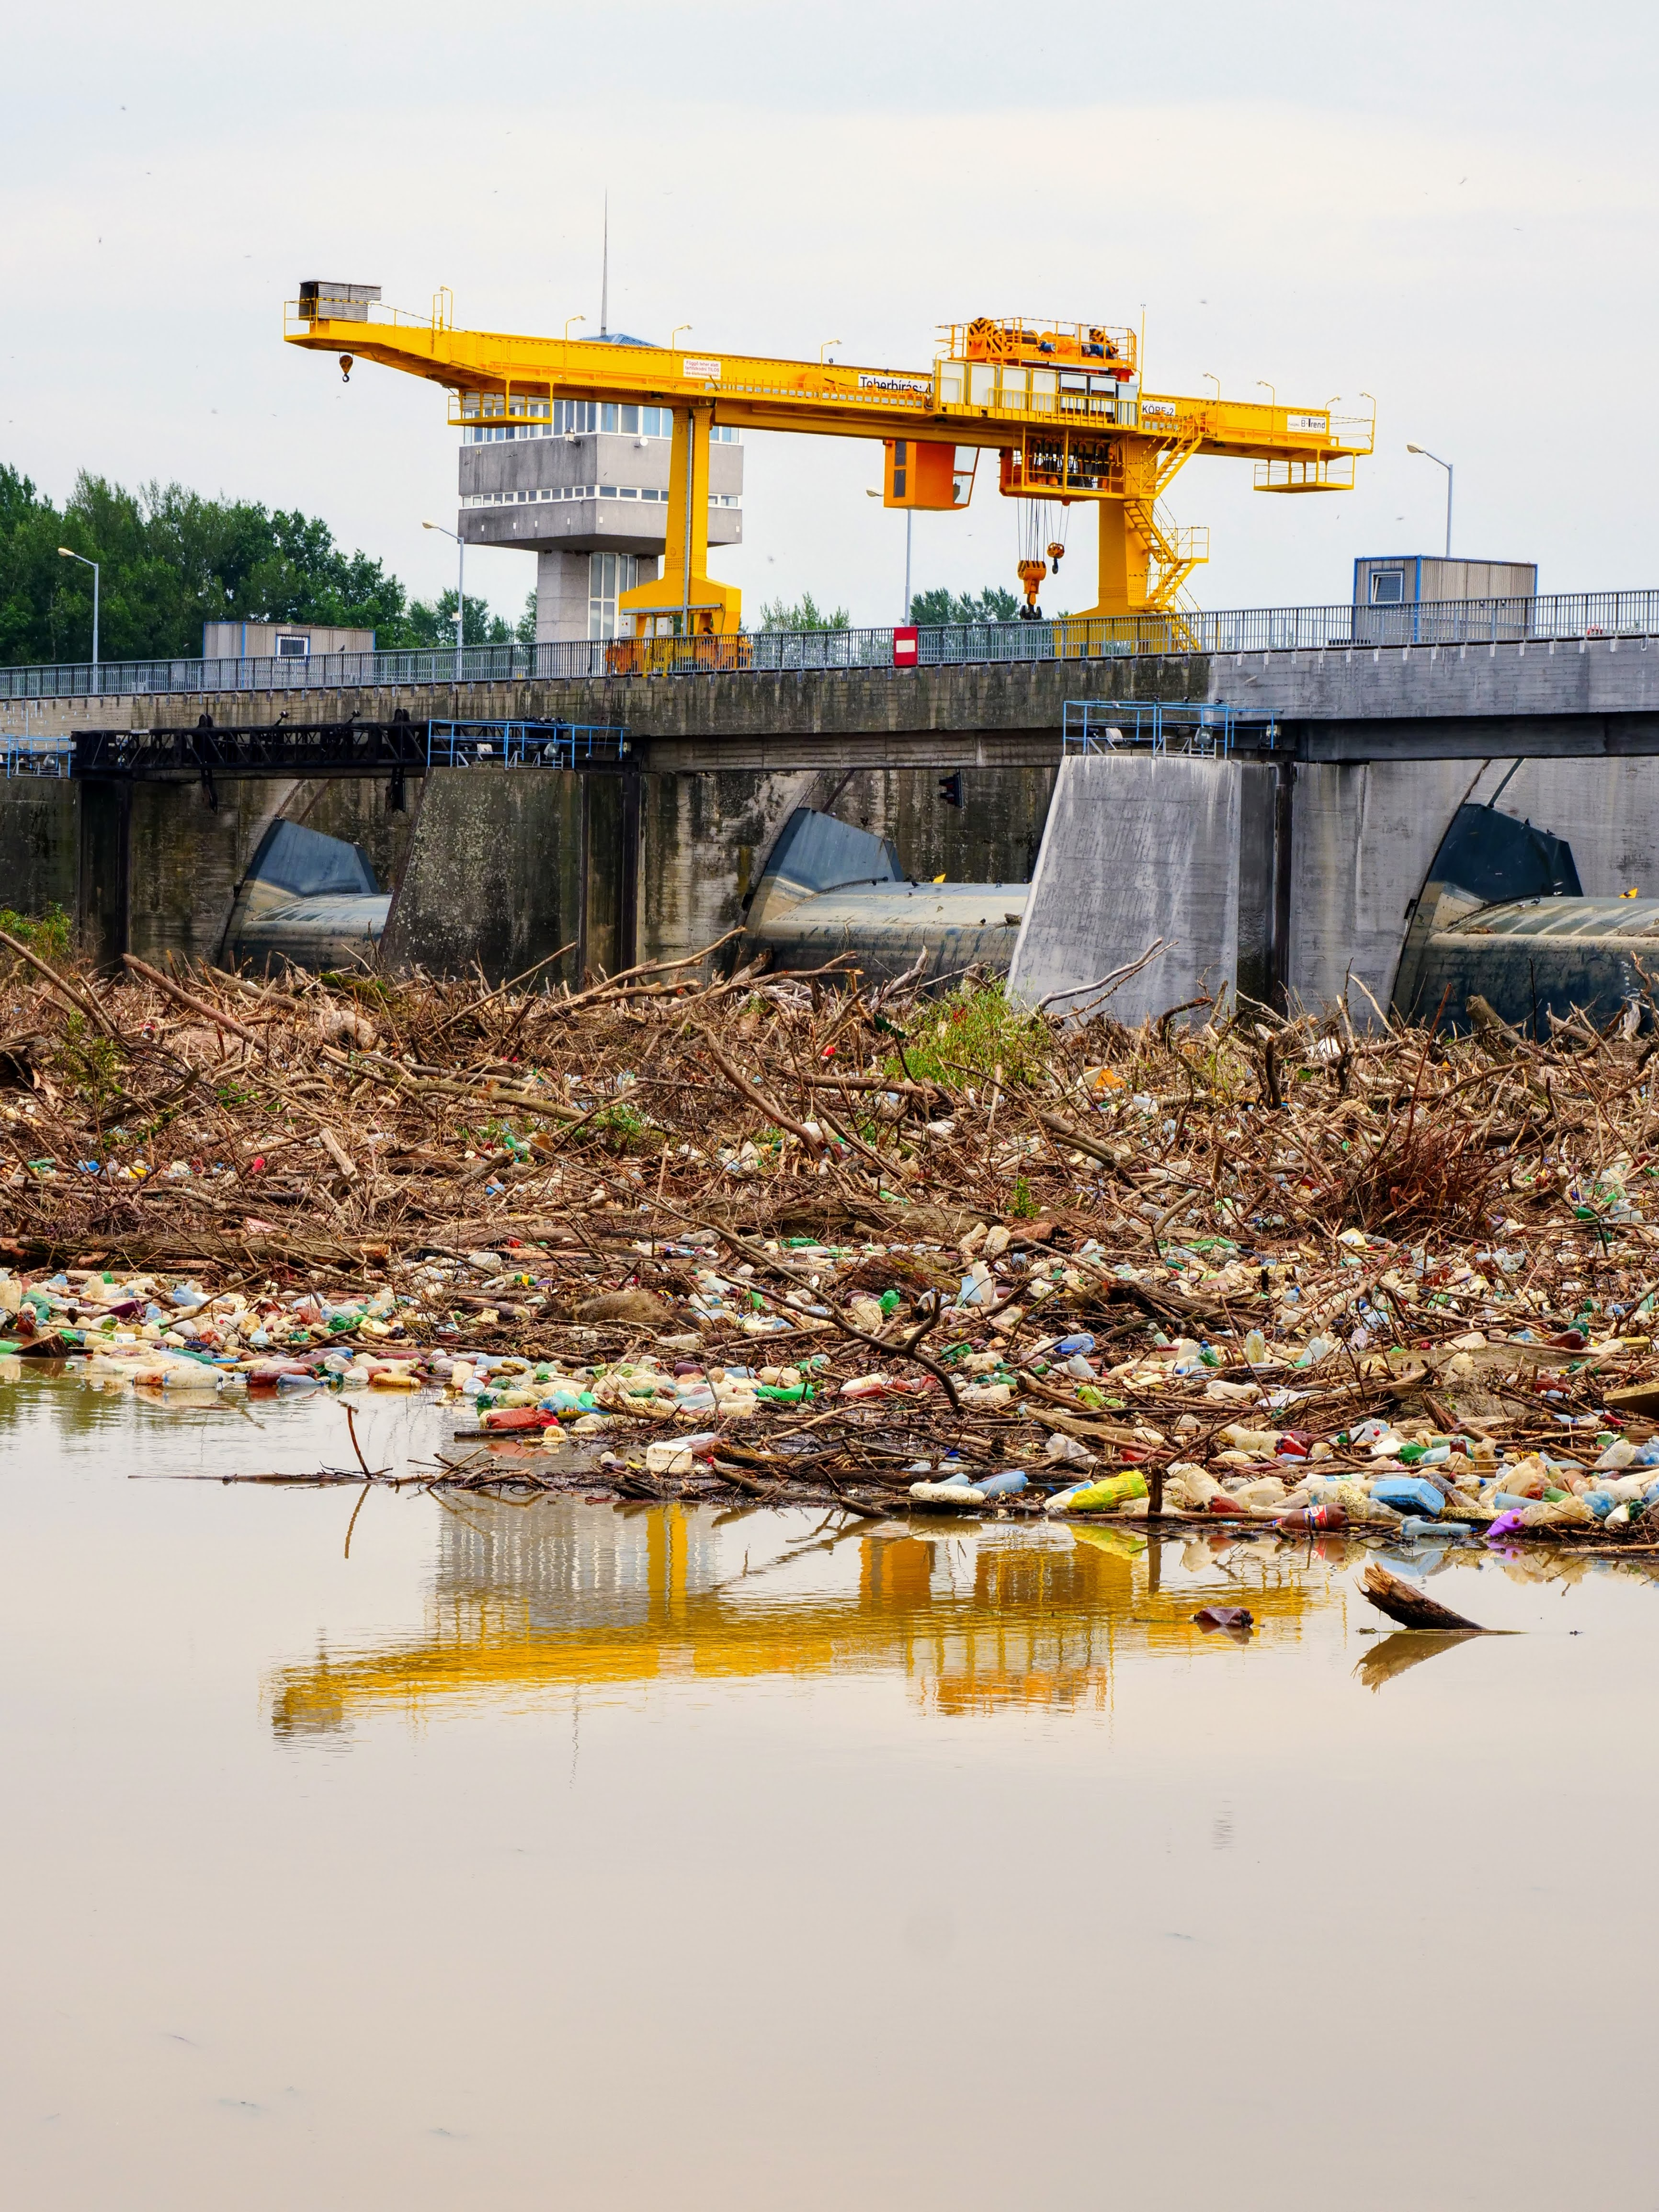
\includegraphics[width=0.6\textwidth,frame]{kiskore-garbage}
	\caption{A kiskörei víztároló hulladéktorlasza \cite{petkupa2024}}
    \label{fig:kiskore-waste}
\end{figure}

\begin{table}[H]
	\centering
	\begin{tabular}{ | p{0.1\textwidth} | p{0.2\textwidth} | p{0.6\textwidth} | }
		\hline
		\textbf{Címke azonosító} & \textbf{Címke neve} & \textbf{Címke magyarázat} \\
		\hline \hline
		\emph{100} & Hulladék & Azon területek, melyeken hulladék van. \\
		\hline
		\emph{200} & Víz & olyan területek, melyeken kizárólag víz van, általában folyók. \\
		\hline
		\emph{300} & Legelők/Erdők & Zöld övezetből álló vad területek. Ezek lehetnek fák lombjai vagy füves zónák. \\
		\hline
        \emph{400} & Mezők & Olyan földes területek, melyek meg vannak művelve, illetve ahol mezőgazdasági növények találhatóak, például gabonafélék. \\
		\hline
        \emph{500} & Ismeretlen & Olyan területek, melyek a korábbi kategóriákba nem sorolhatók bele. Ilyenek az épületek, aszfaltozott utak, háztetők, mezei utak. \\
		\hline
	\end{tabular}
	\caption{A tanítóadatok címkéi}
	\label{tab:waste-detection-labels}
\end{table}

\begin{figure}[H]
	\centering
	\subcaptionbox{Műanyag alapú hulladék}{
		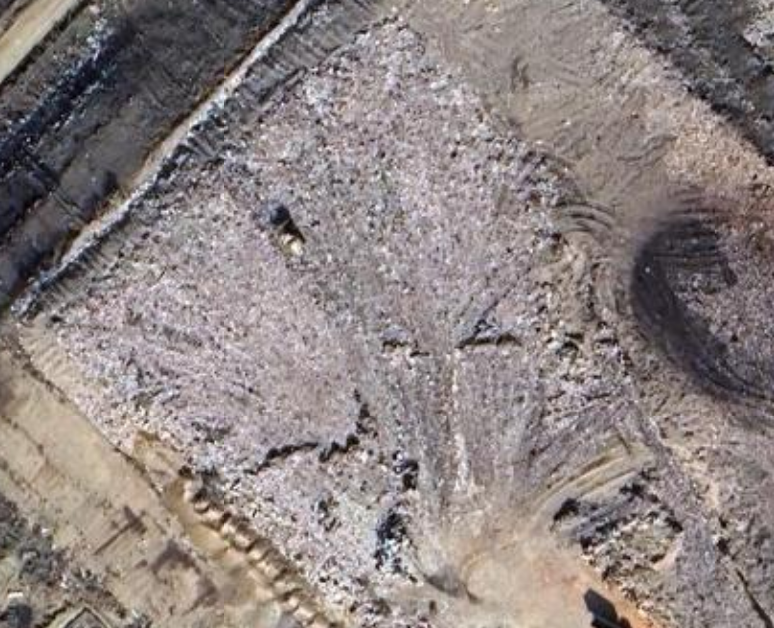
\includegraphics[width=0.45\linewidth]{waste}}
	\hspace{5pt}
	\subcaptionbox{Törmelék}{
		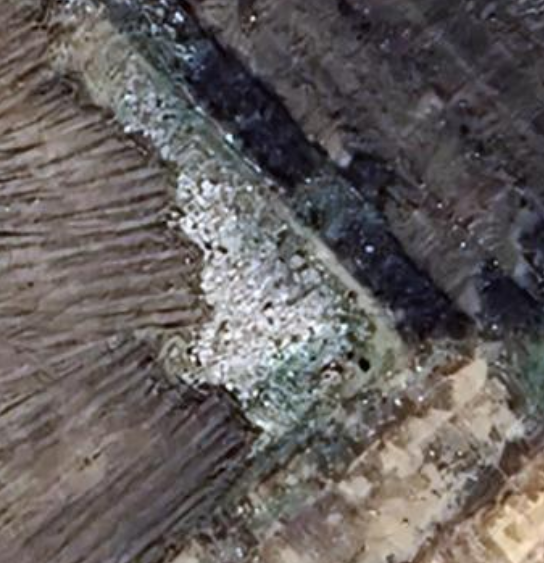
\includegraphics[width=0.45\linewidth]{debris}}
	\caption{A műanyag alapú hulladék, törmelék mellé helyezve. Forrás: Google Maps}
	\label{fig:waste-vs-debris}
\end{figure}



\section{Tanítási paraméterek}
\label{ch:teaching-params}

A Random Forest betanításához a Scikit-Learn Python csomagot használtam \cite{scikit-learn}. A nagy adathalmaz miatt a Random Forest modell is nagyon nagy lett (körülbelül 14GB), ami egy nehezen kezelhető méret, így érdemes módosítani a modell paraméterein, hogy ez kisebb méretű legyen. A legjobb eredményeket azzal értem el, hogy a Random Forest fák méretét 20 mélységűre limitáltam. Ennek köszönhetően a model méretét 2GB-ra tudtam csökkenteni, és a \ref{fig:fullsize-vs-reduced} ábrából látható, hogy a csökkentett modellben enyhén megnő a hulladékra vonatkozó false-negative ráta, míg a false positive arány nem nő, de cserében egy kezelhető méretű modellt kapok.

\begin{figure}[H]
	\centering
  \subcaptionbox{A klasszifikálandó felvétel}{
		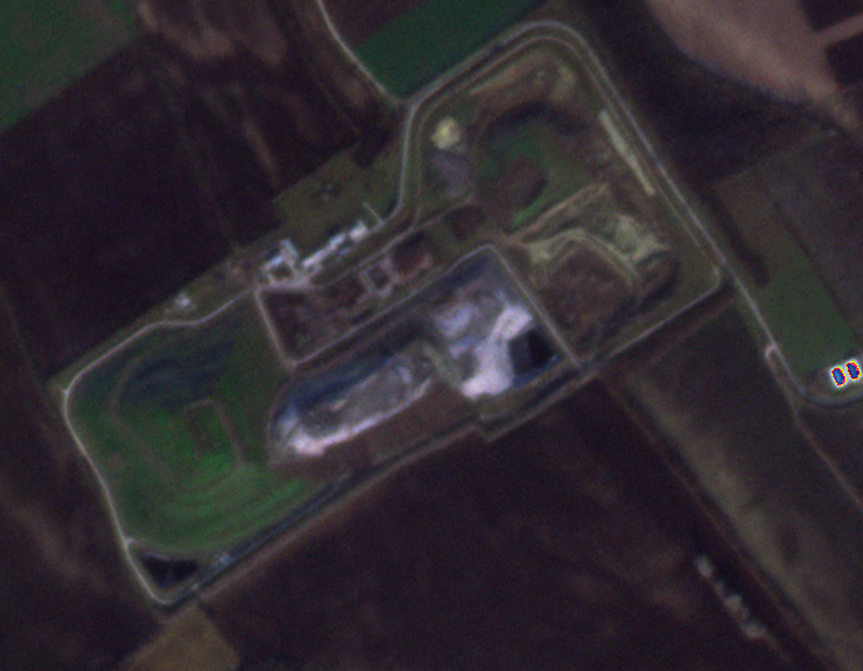
\includegraphics[width=0.45\linewidth]{original-pusztazamor}}
	\hspace{5pt}
	\subcaptionbox{Teljes méretű modell}{
		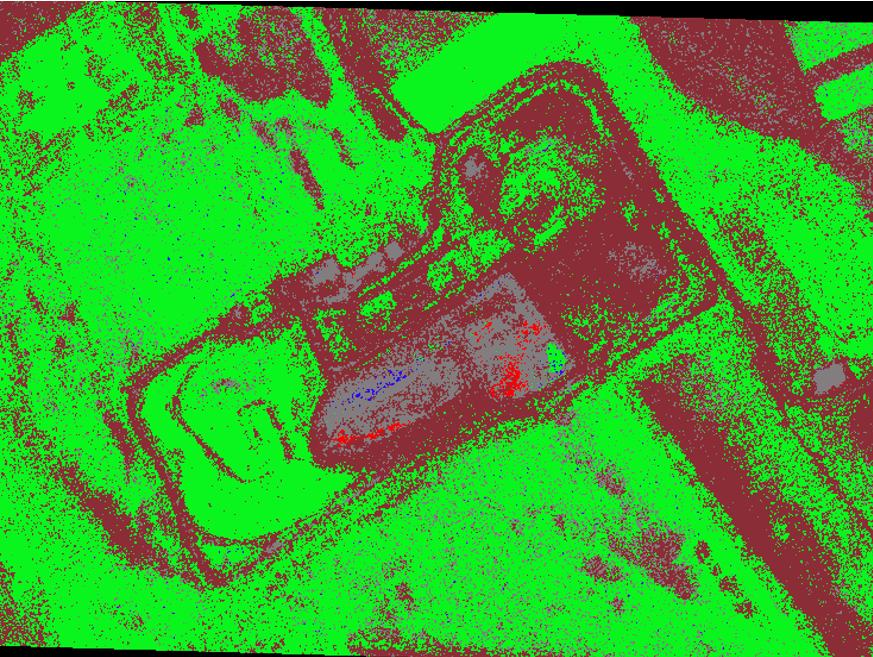
\includegraphics[width=0.45\linewidth]{fullsized}}
	\hspace{5pt}
	\subcaptionbox{Csökkentett modell}{
		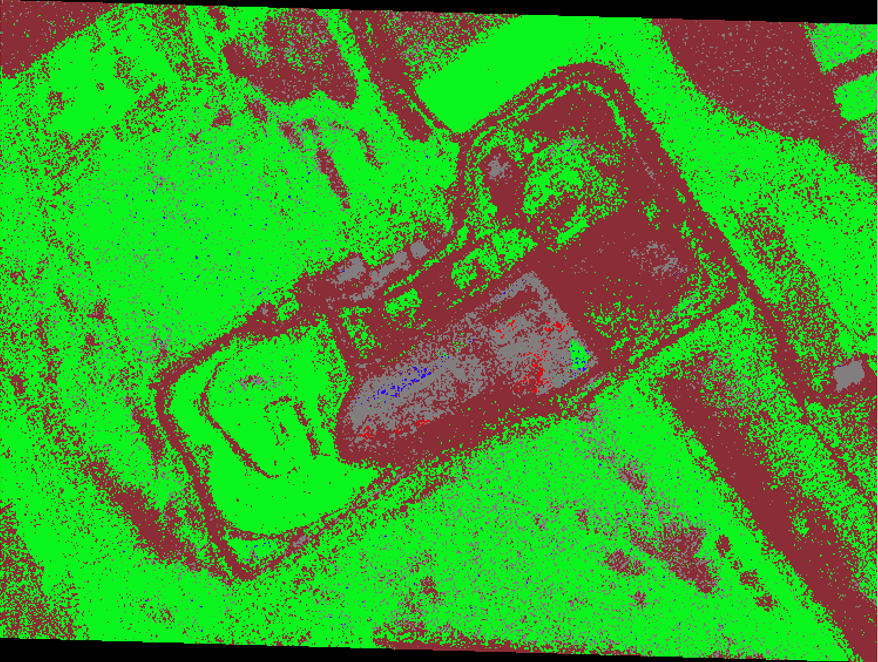
\includegraphics[width=0.45\linewidth]{reduced}}
	\caption{A csökkentett modell hasonlóan teljesít a teljes méretű modellhez}
	\label{fig:fullsize-vs-reduced}
\end{figure}

Továbbiakban felmerült az a probléma is, hogy a tanítóadatok nagyon aránytalanok: A \ref{fig:unbalanced-data} ábrából látható, hogy nagyságrendekkel kevesebb adattal rendelkeztünk hulladékról, mint az összes többi adatról. Emiatt a modell nagyon sok false-negatívot termelt. Ennek korrigálására súlyokat alkalmaztam a tanítóadatokra. A súlyok kiszámolásához az összes címkére a \ref{eq:weights} képletet használtam.

\pgfplotstableread[row sep=\\,col sep=&]{
    label           & value     \\
    Hulladék        & 29513     \\
    Víz             & 926356    \\
    Legelők/Erdők   & 12573615  \\
    Mezők           & 8043948   \\
    Ismeretlen      & 5669416   \\
}\datacounts

\begin{figure}
    \begin{tikzpicture}
        \begin{axis}[
                ybar,
                ymode = log,
                bar width=1cm,
                width=\textwidth,
                height=0.5\textwidth,
                symbolic x coords={Hulladék,Víz,Legelők/Erdők,Mezők,Ismeretlen},
                xtick=data,
            ]
            \addplot table[x=label,y=value]{\datacounts};
        \end{axis}
    \end{tikzpicture}
    \caption{Az adatok közötti aránytalanság, logaritmikus skálázással}
    \label{fig:unbalanced-data}
\end{figure}

\begin{equation}\label{eq:weights}
    c\acute{\imath}mke \ s\acute{u}lya=\frac{adathalmaz \ m\acute{e}rete}{c\acute{\imath}mke \ darabsz\acute{a}ma}
\end{equation}

\section{Felvételek normalizálása}

Az egyik gyakori probléma gépi tanulásban az, hogy ha elég nagy eltérések vannak a felvételek között, például időjárás miatt, akkor a modell hajlandó félreosztályozni egyes területeket. Illetve, a műholdak, amikkel készülnek a felvételek idővel újabb műszereket kapnak, amik eltéréseket termelhetnek a felvételeken. Ennek fényében időben is lehetnek lényeges eltérések a felvételek között. Ennek korrigálára érdemes megvizsgálni a műholdfelvételek normalizálását. A normalizálás egy referencia kép szerint történik: kiválasztok egy referencia felvételt egy adott területről és időszakról (nyár, tél), és az összes többi felvételt arról a területről és időszakról erre a felvételre normalizálom. Így a nagymértékű eltérések csökkentve lesznek a modell számára, és várhatóan jobban fogja osztályozni a felvételeket, amik különböző körülmények között voltak előállítva. A normalizáló algoritmust az ELTE IK térinformatikai laboron belül fejlesztette az egyik kollégám.
A normalizált felvételekhez külön kell egy modellt betanítani. Így a teszthalmazban minden területhez és minden évszakhoz kiválasztottam egy-egy felvételt, mint referencia kép. Ezután minden műholdképet normalizáltam a referenciához. A módszer eredményeit a \ref{ch:normalization-test} fejezetben részletezem.

\section{Főkomponens analízis (PCA)}
\label{ch:pca-methodology}

A modell méretének a csökkentésére megvizsgáltam a főkomponens analízis (PCA) alkalmazását is \cite{pca2010}. A főkomponens analízis a gépi tanulásban egy szélesen elterjedt módszer.  A módszer lényege az, hogy egy többdimenziós adathalmazból kivonja a legfontosabb információkat egy alacsonyabb dimenziószámú adathalmazba. Ezeket nevezzük főkomponenseknek. A főkomponensek korrelálatlanok, vagyis a korrelációs mátrixuknak a főátlóján helyezkednek el, illetve a megfigyelési egységek varianciájának a nagy részét az első pár főkomponensben tároljuk \cite{elek2011}. Azt, hogy hány főkomponenst szeretnénk megtartani, empirikus módon meghatározhatjuk annak függvényében, hogy mekkora mértékben szeretnénk megtartani az eredeti adathalmaz varianciáját. A \ref{fig:pca-variance} ábrán látható, hogy ennek az adathalmaznak az esetében ha 90\%-át szeretném megtartani a varianciának, akkor elég az első három főkomponenst megválasztanom. Így a továbbiakban, minden PCA alkalmazáskor az első három főkomponens kiválasztása értendő.

\pgfplotstableread[row sep=\\,col sep=&]{
    label           & value     \\
    PC1        & 6.673e+01     \\
    PC2             & 2.239e+01    \\
    PC3   & 6.859e+00  \\
    PC4           & 2.032e+00   \\
    PC5     & 1.501e+00    \\
    PC6 & 4.057e-01    \\
    PC7 & 8.222e-02    \\
    PC8 & 5.806e-13    \\
    PC9 & -9.228e-27    \\
}\varianceretention

\begin{figure}
    \begin{tikzpicture}
        \begin{axis}[
                ybar,
                ylabel=megtartott variancia(\%),
                bar width=1cm,
                width=\textwidth,
                height=0.5\textwidth,
                symbolic x coords={PC1,PC2,PC3,PC4,PC5,PC6,PC7,PC8,PC9},
                xtick=data,
            ]
            \addplot table[x=label,y=value]{\varianceretention};
        \end{axis}
    \end{tikzpicture}
    \caption{A főkomponensek varianciája a tanítóhalmazon. 90\% variancia megtartásának érdekében elég az első három főkomponenst kiválasztani}
    \label{fig:pca-variance}
\end{figure}

A PCA használatának a motivációja az volt, hogy a bemeneti adatok dimenziószámának a csökkentésével csökkenni fog a modell mérete, de érdekes módon a modell mérete nem csökkent a dimenziószám csökkentésével, helyette lényegesen megnőtt. Ezt az is tükrözi, hogy megnőtt átlagosan a Random Forest döntési fáinak a mérete, minél kevesebb dimenziószámú adatot kapott. A \ref{tab:increase-in-model-size} táblázatból látható, hogy különböző főkomponenseknél mekkora volt átlagban a fák mérete az adatok dimenziószámának függvényében. További vizsgálatok után kiderült, hogy hogyha kevesebb dimenziójú adatot adtam a modellnek, akkor a mérete lényegesen megnőtt. 

Ezen felül az is célja volt a PCA alkalmazásának, hogy a kiszámolt indexek információit megtartva, alacsonyabb dimenziószám segítségével a Random Forest modell hatékonyabban fogja majd feldolgozni a műholdfelvételeket. \cite{Howley2005} megmutatja, hogy egyes modelleken jobb klasszifikációt tudtak elérni több spektrális sávból álló adat esetén. Ennek az az oka, hogy ha igen sok a korreláció a különböző dimenziók között, akkor a modell rátanulhat a zajra. Mivel a modell által használt indexek között sok a korreláció, érdemes megvizsgálni a PCA-t olyan szempontból is, hogy esetleg javít-e a klasszifikációs eredményeken. 

\begin{table}[H]
	\centering
	\begin{tabular}{ | p{0.3\textwidth} | p{0.3\textwidth} | }
		\hline
		\textbf{Főkomponensek száma} & \textbf{Fák méretének mediánja} \\
		\hline \hline
		Főkomponensek nélkül (9 dimenzió) & 71.5 \\
		\hline
    5 főkomponens & 71 \\
		\hline
		4 főkomponens & 73\\
		\hline
    3 főkomponens & 85 \\
    \hline
	\end{tabular}
	\caption{A döntési fák méretének a mediánja nem csökkent, amint a főkomponensek száma csökkent, cserében 3 főkomponensnél már nőtt.}
	\label{tab:increase-in-model-size}
\end{table}

A PCA alkalmazása a Random Forestre a következő lépésekből áll:
\begin{enumerate}
	\item A tanítóadatok standard skálázása a \ref{eq:standard-scaling} képlet szerint.
	\item A főkomponens analízis alkalmazása a tanítóadatokra.
	\item A Random Forest modell betanítása a tanítóadatokon.
\end{enumerate}
A főkomponens analízis folyamatának a geometriai jelentését a \ref{fig:elek-pca} ábra illusztrálja.

\begin{equation}\label{eq:standard-scaling}
  f(x) = \frac{x - Average}{Standard \ Deviation}
\end{equation}

\begin{figure}[H]
	\centering
	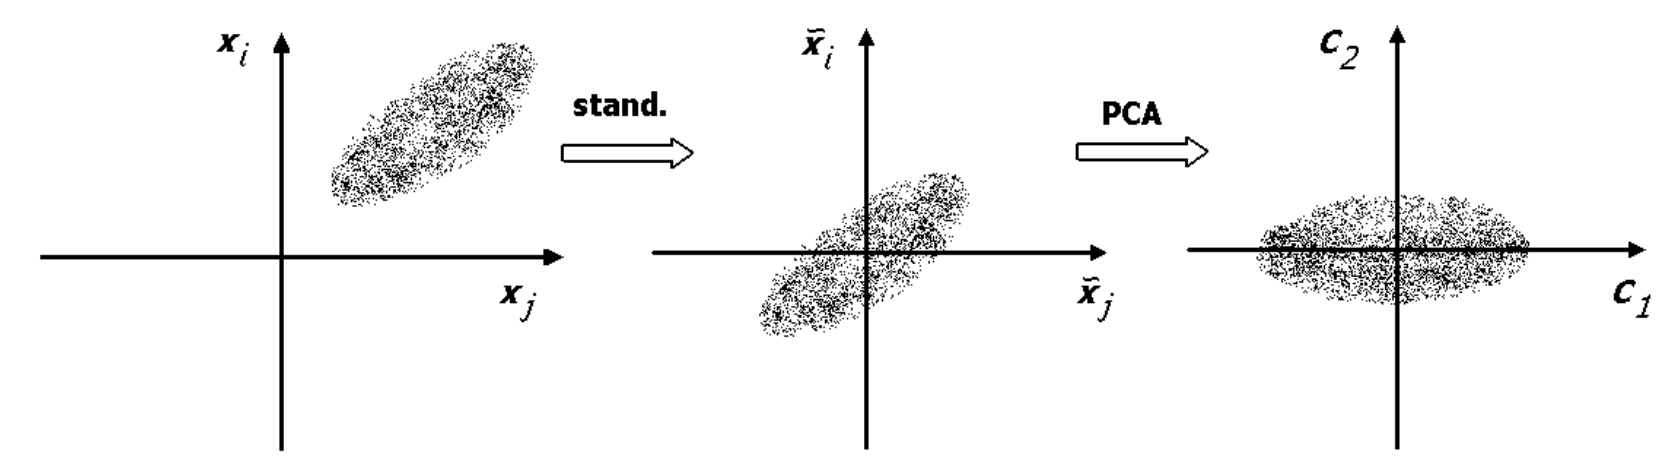
\includegraphics[width=\textwidth,frame]{elek_pca}
	\caption{A főkomponens analízis geometriai jelentése: a standardizálás 0 várható értékűvé és
  1 empirikus szórásúvá teszi a változókat, vagyis a pontfelhőt betolja az origóba,
  majd elforgatja a legnagyobb variancia irányába, ami az első főkomponens \cite{elek2011}}
    \label{fig:elek-pca}
\end{figure}

A modell tesztelésére is ugyanezeket a lépéseket kell elvégezni. A főkomponens analízis használásához a scikit-learn \cite{scikit-learn} Python programcsomagot használtam. A főkomponens analízissel betanított modellt a \ref{ch:teaching-params} fejezetben leírtak szerint paramétereztem. A \ref{ch:pca-performance} fejezetben részletezem a főkomponens analízissel tanított modell teljesítményét.

\section{Nyári és téli adatokra való lebontás}

Alapértelmezetten a nyári és téli adatok között lényeges különbség tud lenni távérzékelés szempontból Közép-Európa területén: a téli időszakokban gyérebb a vegetáció, ködösebb a levegő, illetve a nap sem süt ugyanabból a szögből. Ez befolyásolhatja a modell pontosságát is az adott időszakokban. A nyári időszakot márciustól októberig tartó időszakként definiáltam, és a téli időszak pedig novembertől februárig tart. Az időszakok aszerint vannak megválasztva, hogy mikor leveleznek ki, illetve hullatják ki a leveleiket a fák. Valóban, az októberi időszakban már inkább sárgásak lesznek a levelek, de az októberi tanítóhalmaz mérete önmagában igen kicsi érdemi tanításra. A \ref{fig:winter-vs-summer} ábrából látható, hogy főleg a közeli infravörös (NIR) sávokon nagy eltérések vannak a nyári és téli felvételek között. Ennek fényében betanítottam külön egy nyári és egy téli modellt, melyek teljesítményét a \ref{ch:summer-winter-models} fejezetben részletezem.

\begin{figure}
    \begin{tikzpicture}
        \begin{axis}
          [
          title={Téli felvételek értékei},
          boxplot/draw direction=y,
          ytick={0,2000,4000,6000},
          ymax={8000},
          xtick={1,2,3,4},
          xticklabels={Kék, Zöld, Piros, NIR},
          ]
          \addplot+[
          boxplot prepared={
            median=428,
            upper quartile=563,
            lower quartile=315,
            upper whisker=935,
            lower whisker=44
          },
          ] coordinates {};
          \addplot+[
          boxplot prepared={
            median=530,
            upper quartile=695,
            lower quartile=385,
            upper whisker=1160,
            lower whisker=1
          },
          ] coordinates {};
          \addplot+[
          boxplot prepared={
            median=674,
            upper quartile=923,
            lower quartile=497,
            upper whisker=1562,
            lower whisker=22
          },
          ] coordinates {};
          \addplot+[
            boxplot prepared={
              median=1629,
              upper quartile=2067,
              lower quartile=1273,
              upper whisker=3258,
              lower whisker=82
          },
          ] coordinates {};
        \end{axis}
      \end{tikzpicture}
      \begin{tikzpicture}
        \begin{axis}
          [
          title={Nyári felvételek értékei},
          boxplot/draw direction=y,
          ytick={0,2000,4000,6000},
          ymax={8000},
          yticklabel=\empty,
          xtick={1,2,3,4},
          xticklabels={Kék, Zöld, Piros, NIR},
          ]
          \addplot+[
          boxplot prepared={
            median=360,
            upper quartile=638,
            lower quartile=214,
            upper whisker=1274,
            lower whisker=1
          },
          ] coordinates {};
          \addplot+[
          boxplot prepared={
            median=578,
            upper quartile=862,
            lower quartile=415,
            upper whisker=1532,
            lower whisker=1
          },
          ] coordinates {};
          \addplot+[
          boxplot prepared={
            median=579,
            upper quartile=1058,
            lower quartile=270,
            upper whisker=2240,
            lower whisker=1
          },
          ] coordinates {};
          \addplot+[
            boxplot prepared={
              median=2850,
              upper quartile=3830,
              lower quartile=2103,
              upper whisker=6420,
              lower whisker=1
          },
          ] coordinates {};
        \end{axis}
      \end{tikzpicture}
    \caption{Nyári és téli adatok összehasonlítása}
    \label{fig:winter-vs-summer}
\end{figure}
\cleardoublepage

\chapter {Verifikáció}
\label{ch:verification}

\section{A teszthalmaz}
\label{ch:test-set}

A teszthalmaz 3 nyári drinai felvételből áll, ahol a hulladékkal szennyezett területeket kézzel annotáltam. Ez a terület egyben egy szárazföldi hulladéklerakót (\ref{fig:drina-deposit} ábra), illetve egy vízfelszíni hulladékszigetet is tartalmaz, így alkalmas mindkét detektálásnak a tesztelésére. A \ref{fig:drina-floating-waste} ábrából látható, hogy Drinán úgy fogják meg az úszó műanyag-alapú hulladékot, hogy egy zsinórra ráhúznak üres hordókat, melyek a víz felszínén lebegnek. Így, minden, ami elég könnyű ahhoz, hogy a folyó felszínen ússzon (műanyagpalackok, kisebb fadarabok) megakad a hordók mögött, míg például nagyobb fadarabok, vagy más, nehezebb uszadékok a zsinór alatt elúsznak. Így a folyó felszínén kialakuló sziget nagy koncentrációban tartalmaz műanyag alapú hulladékot, tehát alkalmas arra, hogy a modellt ezen validáljam vízfelszíni hulladékdetektáláshoz. Ráadásul erről a területről nem készültek tanító adatok ebben a kutatásban, így a modell teljesítménye az itteni felvételeken jól tesztelhető. A téli drinai és nyári kiskörei felvételek a \ref{ch:empirical-validation} fejezetben vannak vizsgálva.

A \ref{fig:old-vs-new} ábrából látható egy-egy vizuális összehasonlítás a régi és az új modell klasszifikációja között a teszthalmaz egyik felvételén. A hulladékos területek pirossal vannak jelölve. Látszik ezen a példán, hogy az új modell több \textit{false negative}-ot\todo[color=blue!50]{A magyar szövegben az angol kifejezéseket érdemes tipográfiailag kiemelni, pl. dőlten szedni. Botond: Rendben, a false positive, negative-okat átírtam, ha még találok ilyet a szövegben, azokat is átírom} termel főleg a hulladéksziget körül, de ugyanakkor lényegesen lecsökkenti a \textit{false positive}-ok arányát a régi modellhez képest. Ráadásul a folyó mellett található hulladéklerakót is megtalálja az új modell, míg a régi modell nem találja meg, ellenben a lerakó környékét és az utakat, épületeket gyakran hulladéknak detektálja. Ez egy fontos eredmény, hiszen amint a \ref{ch:goals} fejezetben is tárgyaltam, célja ennek a kutatásnak, hogy csökkentsem a modell \textit{false positive} arányait, miközben továbbra is meg tudja találni a hulladéklerakókat, illetve hulladékszigeteket.

\begin{figure}[H]
	\centering
	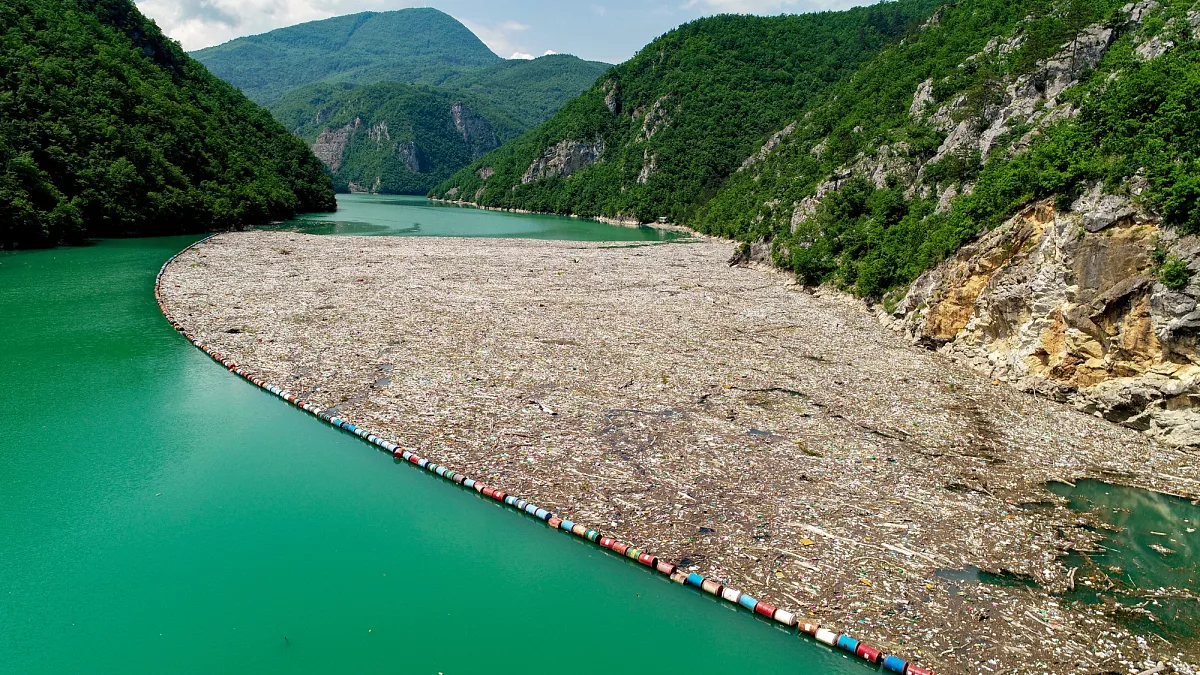
\includegraphics[width=0.6\textwidth,frame]{drina_waste}
	\caption{A drinai hulladéksziget. Egy lebegő zsinór fogja meg a műanyagpalackokat \cite{euronews2024}}
    \label{fig:drina-floating-waste}
\end{figure}

\begin{figure}[H]
	\centering
	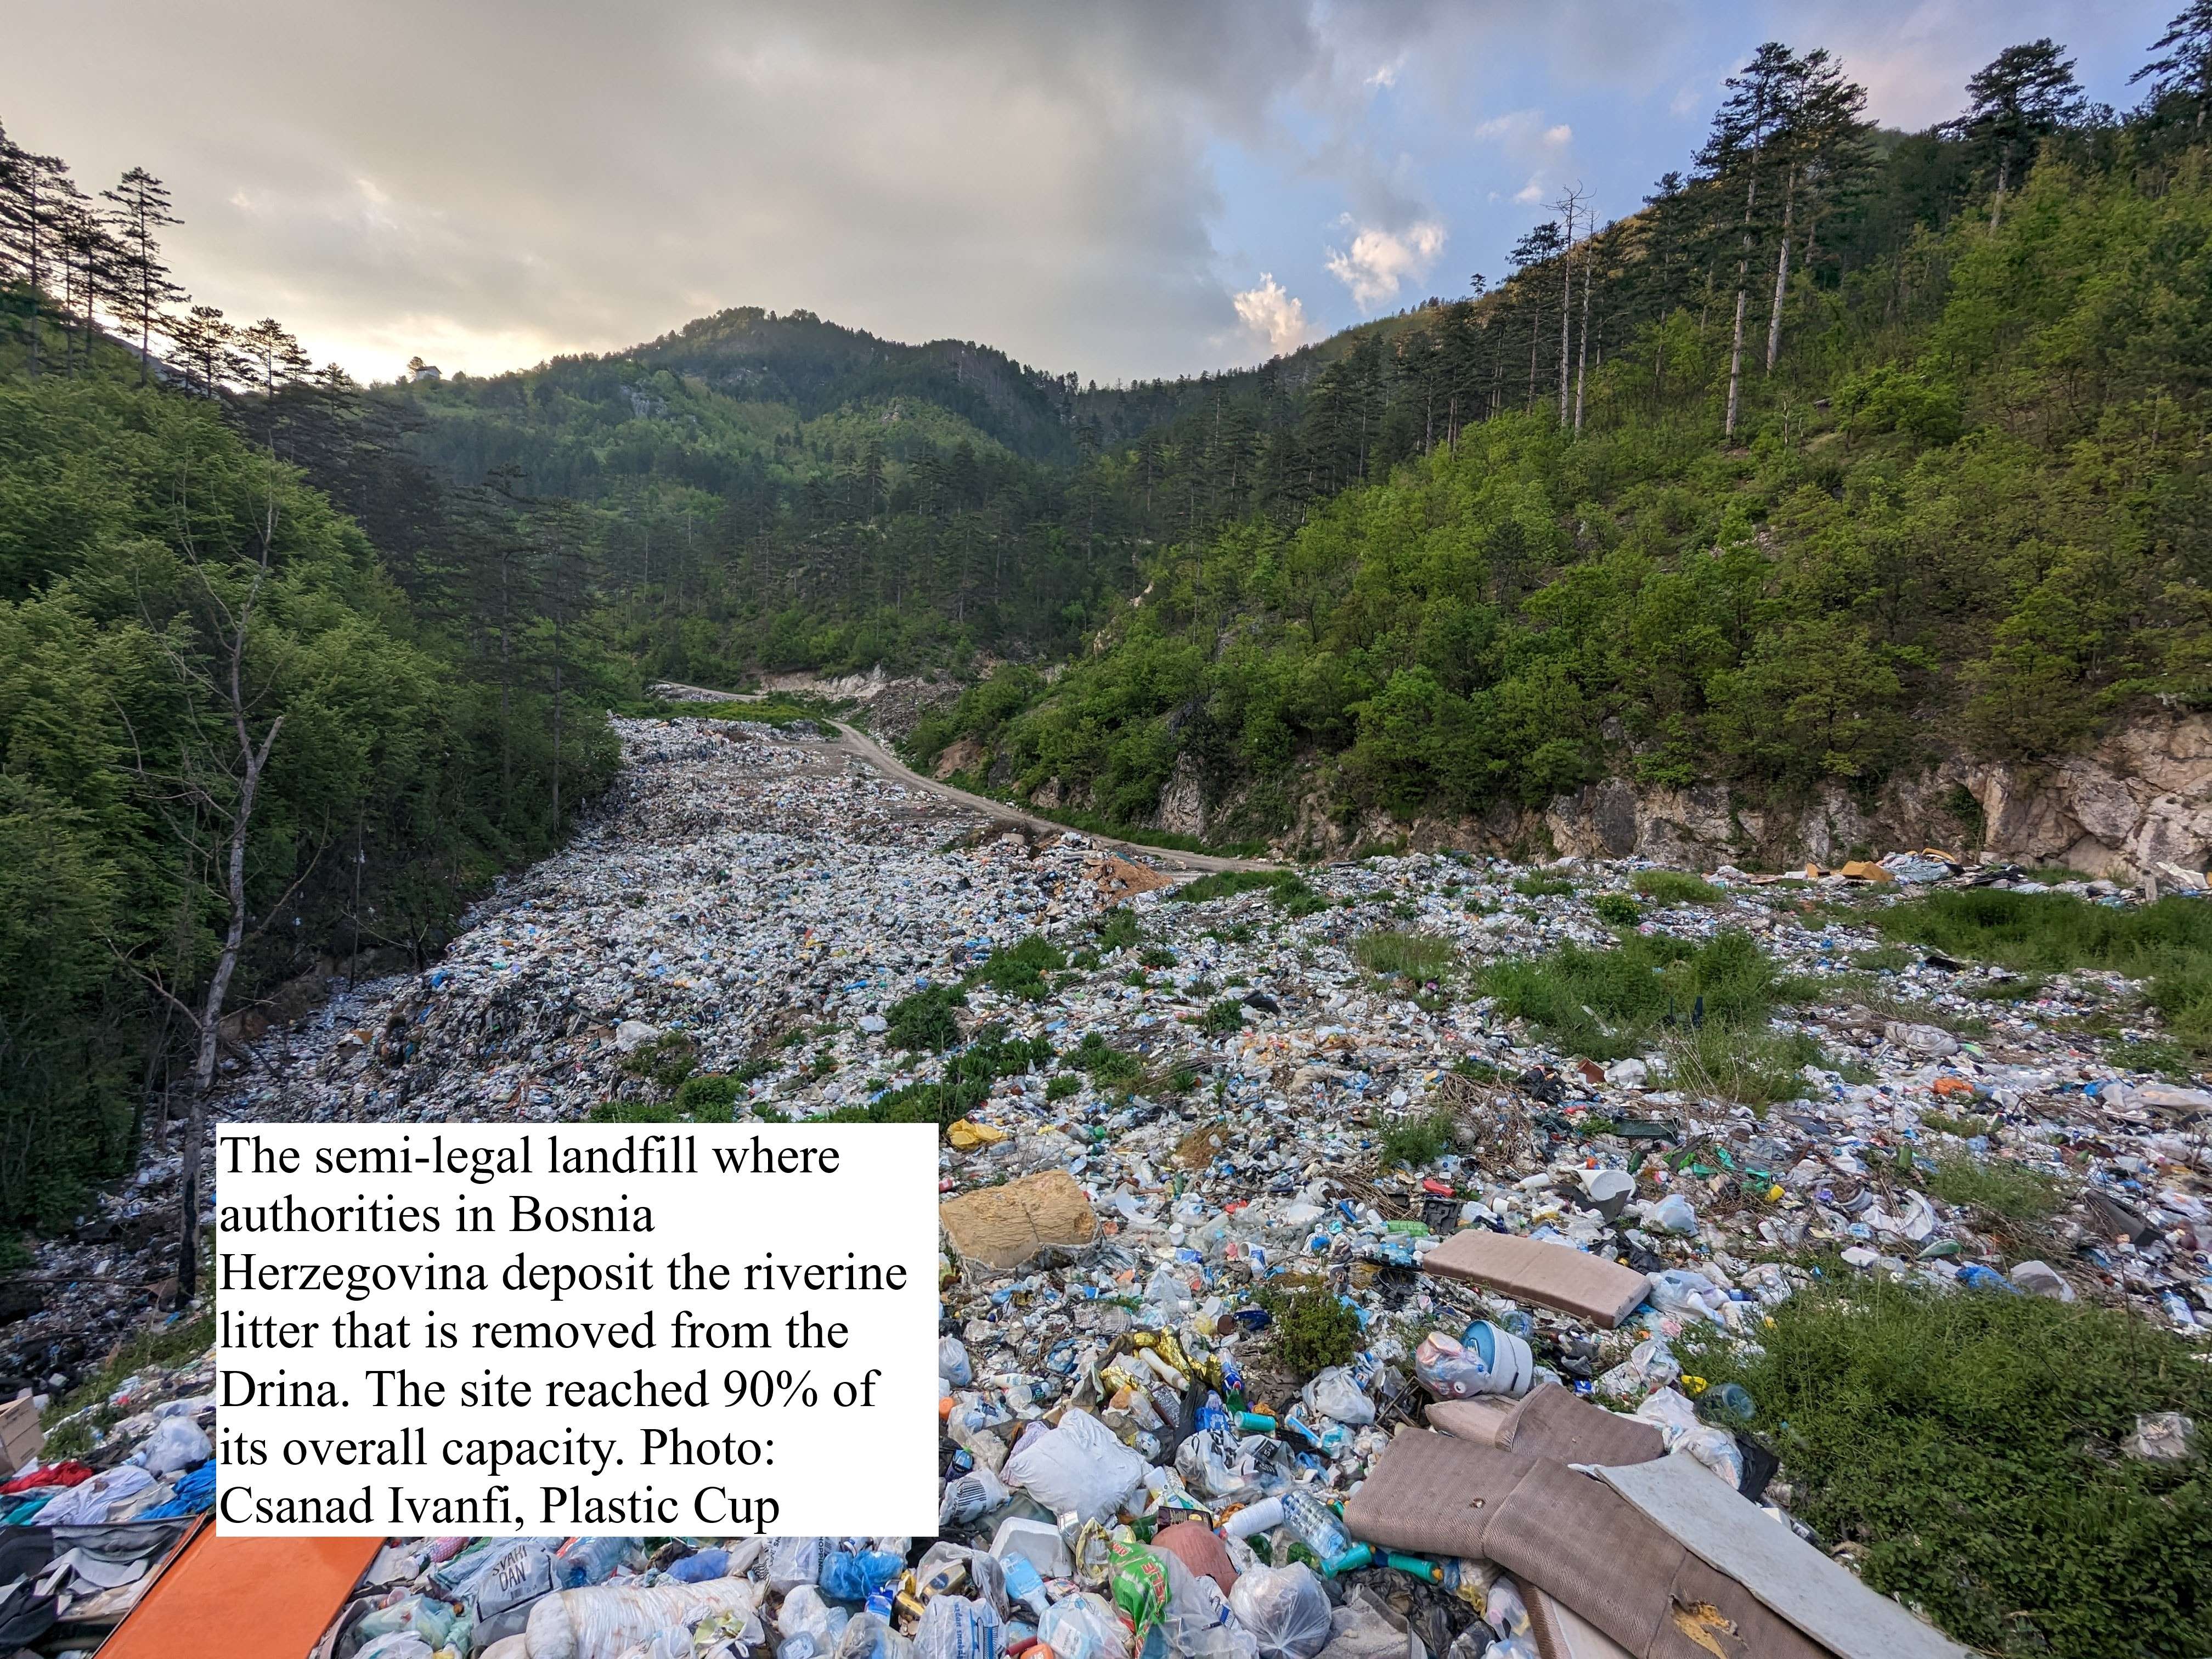
\includegraphics[width=0.6\textwidth,frame]{drina_deposit}
	\caption{A Drina melletti féllegális szemétlerakó \cite{petkupa2024}}
    \label{fig:drina-deposit}
\end{figure}

\begin{figure}[H]
	\centering
  \subcaptionbox{A teszthalmaz kézi annotációja}{
		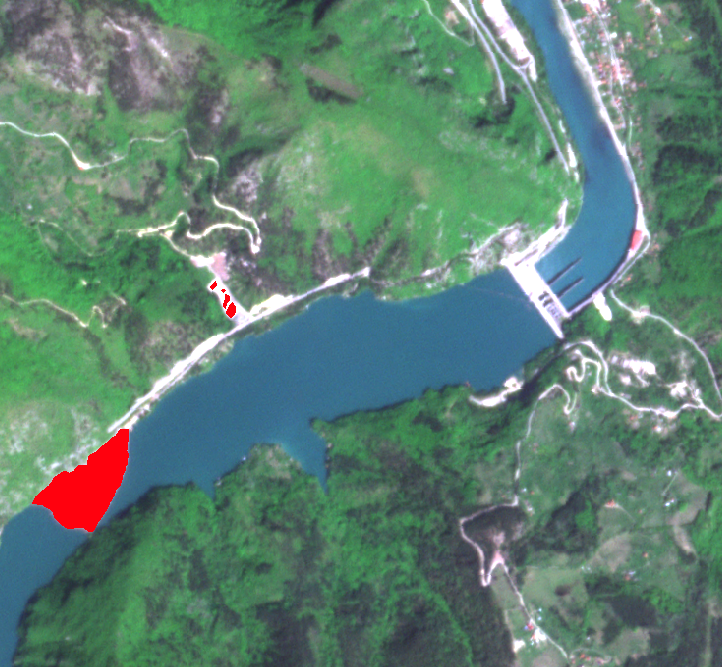
\includegraphics[width=0.45\linewidth]{drina-test}}
	\hspace{5pt}
	\subcaptionbox{A teszthalmaz annotációja a régi modellel}{
		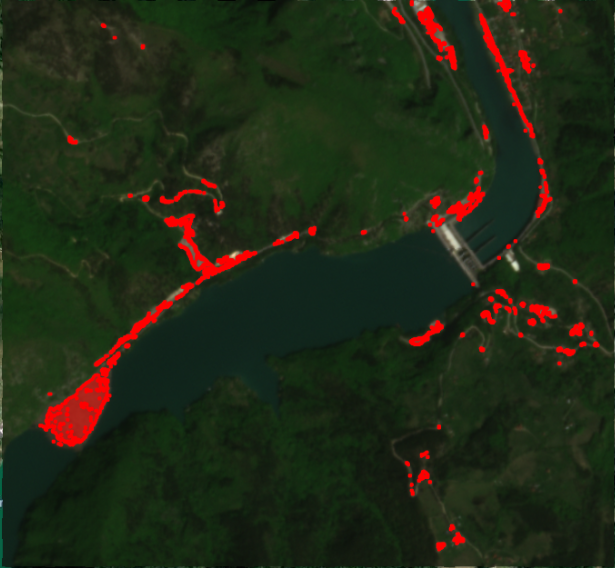
\includegraphics[width=0.45\linewidth]{drina-old}}
	\hspace{5pt}
	\subcaptionbox{A teszthalmaz annotációja az új modellel}{
		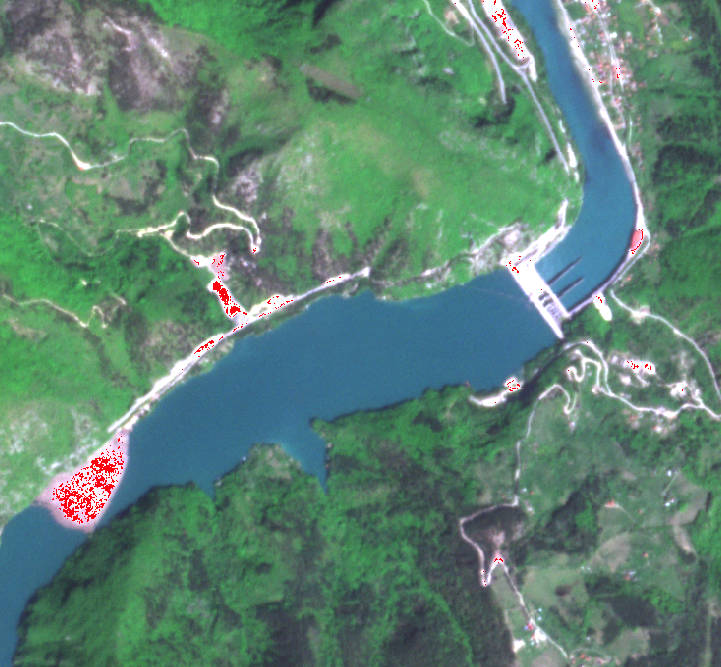
\includegraphics[width=0.45\linewidth]{drina-new}}
	\caption{Az új modell összehasonlítása a régi modellel az egyik Drinai teszt felvételen. Felvétel dátuma: 2023.05.07.}
	\label{fig:old-vs-new}
\end{figure}
\todo[color=blue!50]{Ez és a többi Drinás kép nagyon sötét. Jó lenne kicsit világosítani a hátteren, akár Photoshoppal :). Botond: kivilágosítottam.}

\section{Teljesítmény mérése}

A teszthalmaz eredményeit a "Confusion Matrix" módszerével értékeltem ki \cite{CONGALTON199135}. Ezután ezeket az értékeket arra használtam, hogy a "Comission rate" (\ref{eq:comission-rate} képlet), "Omission rate" (\ref{eq:omission-rate} képlet), "Match rate" (\ref{eq:match-rate} képlet), illetve "Extraction rate" (\ref{eq:extraction-rate} képlet) értékeket számítsam ki \cite{Fekete2021}.

\begin{equation}\label{eq:comission-rate}
    Comission \ rate = \frac{N_{com}}{N_{ref}}
\end{equation}

\begin{equation}\label{eq:omission-rate}
    Omission \ rate = \frac{N_{om}}{N_{ext}}
\end{equation}

\begin{equation}\label{eq:match-rate}
    Match \ rate = \frac{N_{match}}{N_{ref}}
\end{equation}

\begin{equation}\label{eq:extraction-rate}
    Extraction \ rate = \frac{N_{ext}}{N_{ref}}
\end{equation}

$N_{com}$, $N_{om}$, $N_{match}$, $N_{ext}$, $N_{ref}$, rendre a \textit{false positive}, \textit{false negative} (A mátrix mellékátlói), \textit{true positive} (A mátrix főátlója), a modell által detektált pozitív, illetve a referencia adatokban található positív értékek. Összehasonlítottam az új modell teljesítményét a régi modell teljesítményével. A \ref{tab:old-vs-new} táblázatból látható a két modell teljesítményének az átlaga a három felvételen.

\begin{table}[H]
	\centering
	\begin{tabular}{ | p{0.33\textwidth} | p{0.33\textwidth} | p{0.33\textwidth} | }
		\hline
		\textbf{Mérés azonosító} & \textbf{Régi modell átlagai (\%)} & \textbf{új modell átlagai (\%)} \\
		\hline \hline
		\emph{Comission Rate} & 63.67 & 28.13 \\
		\hline
		\emph{Omission Rate} & 26.21 & 70.67 \\
		\hline
		\emph{Match Rate} & 73.79 & 29.32 \\
		\hline
        \emph{Extraction Rate} & 208.18 & 41.31 \\
		\hline
	\end{tabular}
	\caption{A régi modell és az új modell teszteredményei átlagolva}
	\label{tab:old-vs-new}
\end{table}

Az új modell egy jóval kisebb \textit{false postive} aránnyal rendelkezik mint a régi modell, de cserében a \textit{false negative} arányok is nagyok. Ennek oka a \ref{fig:old-vs-new} ábrából látható, hiszen a régi modell sokkal több pontot detektál a hulladékszigeten, míg az új modell kevesebb pontot detektál, de továbbra is nagy mértékben megtalálja a hulladékszigetet. Illetve a \ref{ch:test-set} fejezetben is tárgyaltam, hogy a szárazföldi hulladéklerakót a folyó mellett az új modell már megtalálja, míg a régi nem találja meg. Tekintve arra, hogy a match rate a true positive-al arányos, és az Extraction rate az összes pozitive-al arányos, ezek az értékek is kisebbek lesznek, mint a régi modell értékei.

\section{Főkomponens analízis teljesítménye}
\label{ch:pca-performance}

A \ref{ch:pca-methodology} fejezetben részletezett főkomponens analízis módszert is összehasonlítottam az új modell teljesítményével, a Confusion Matrix módszerének segítségével. A \ref{fig:pca-vs-no-pca} ábrából látható, hogy a főkomponens analízissel tanított modell sokkal jobban ki tudja szűrni a vízfelszínen kialakuló zajt. Az is látható, hogy a főkomponens analízissel kombinált Random Forest is hasonlóan tudja detektálni a hulladékkal szennyezett területeket, annyi különbséggel, hogy a hulladékos területen több pontot detektál, de cserében több false-positive-ot termel.

\begin{figure}[H]
	\centering
  \subcaptionbox{A teszthalmaz kézi annotációja}{
		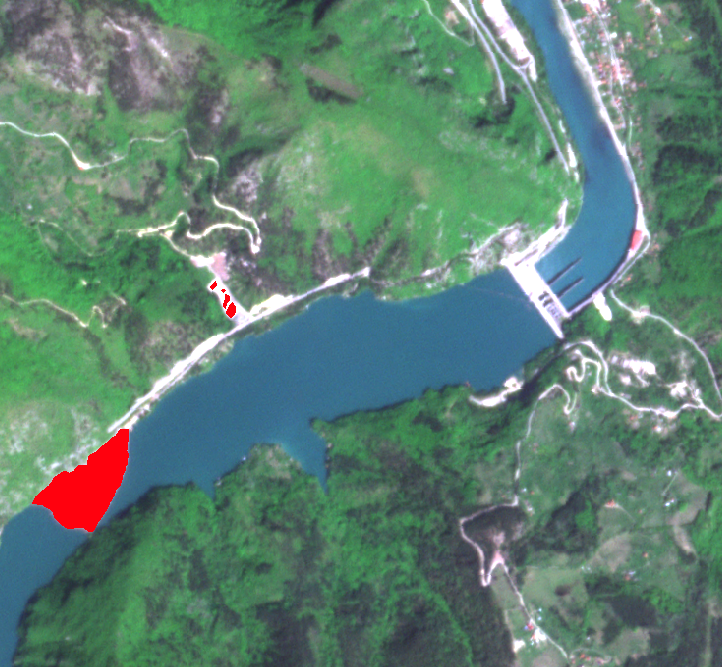
\includegraphics[width=0.45\linewidth]{drina-test}}
	\hspace{5pt}
	\subcaptionbox{A teszthalmaz annotációja az új modellel}{
		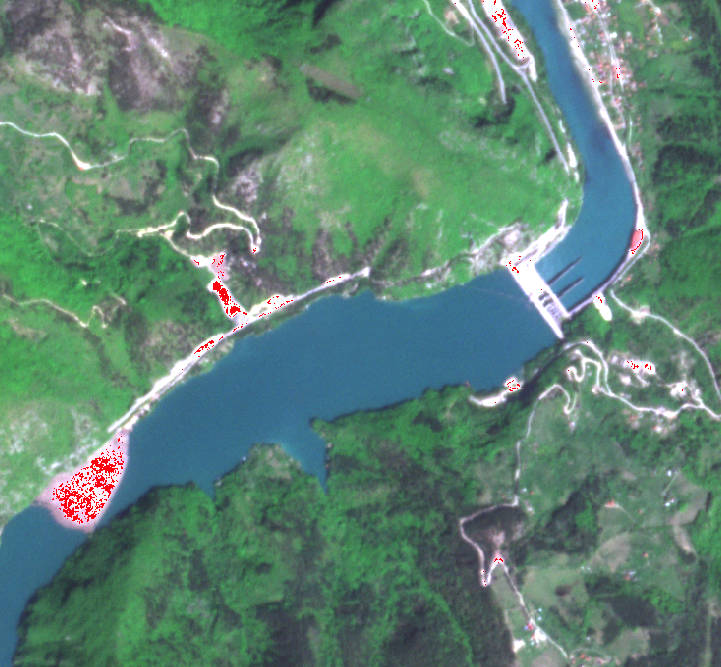
\includegraphics[width=0.45\linewidth]{drina-new}}
	\hspace{5pt}
	\subcaptionbox{A teszthalmaz annotációja az új modellel, PCA segítségével}{
		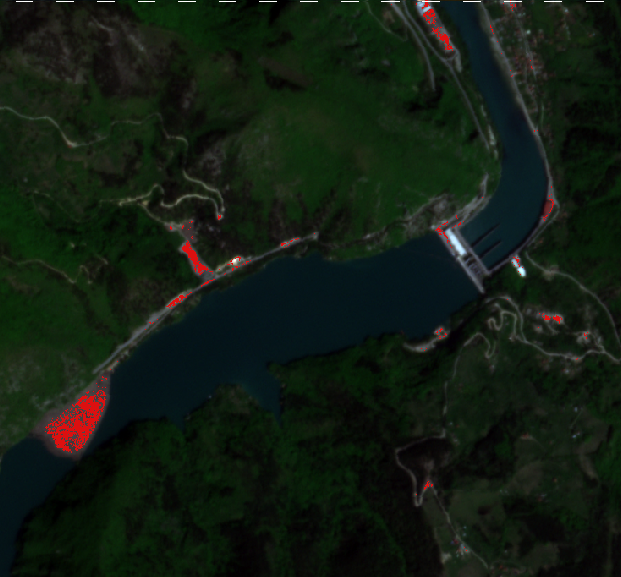
\includegraphics[width=0.45\linewidth]{drina-with-pca}}
	\caption{Az új modell összehasonlítása a PCA-val tanított modellel az egyik Drinai teszt felvételen. Felvétel dátuma: 2023.05.07.}
	\label{fig:pca-vs-no-pca}
\end{figure}

A \ref{tab:pca-vs-no-pca} táblázatban összesítem a főkomponens analízis mutatóit. A táblázatból leolvasható, hogy míg a főkomponens analízis picivel nagyobb \textit{false positive} aránnyal rendelkezik, egyben kisebb \textit{false negative} aránnyal rendelkezik. Ráadásul a felvételeken készülő zajt sokkal jobban kezeli, amint a \ref{fig:classification-pca-vs-no-pca} ábrából is látható: A főkomponens analízissel betanított modell sokkal jobban tudta detektálni a vizet a folyón, mint a főkomponens analízis nélküli modell.

\begin{table}[H]
	\centering
	\begin{tabular}{ | p{0.33\textwidth} | p{0.33\textwidth} | }
		\hline
		\textbf{Mérés azonosító} & \textbf{PCA-val tanított modell átlagai (\%)} \\
		\hline \hline
		\emph{Comission Rate} & 39.01 \\
		\hline
		\emph{Omission Rate} & 65.00 \\
		\hline
		\emph{Match Rate} & 34.99  \\
		\hline
        \emph{Extraction Rate} & 65.25 \\
		\hline
	\end{tabular}
	\caption{A főkomponens analízissel betanított modell teljesítményének az átlagai}
	\label{tab:pca-vs-no-pca}
\end{table}\todo[color=blue!50]{Mellé raknám a PCA nélküli eredményeket, a könnyebb összevethetőség érdekében.}

\begin{figure}[H]
	\centering
  \subcaptionbox{Drina műholdfelvétele}{
		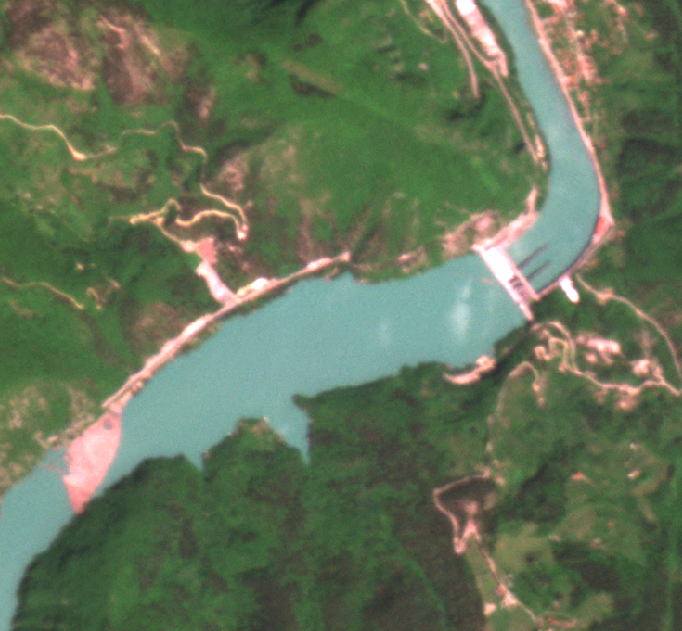
\includegraphics[width=0.45\linewidth]{drina20230521}}
	\hspace{5pt}
	\subcaptionbox{A PCA nélküli modell címkézése a Drinán}{
		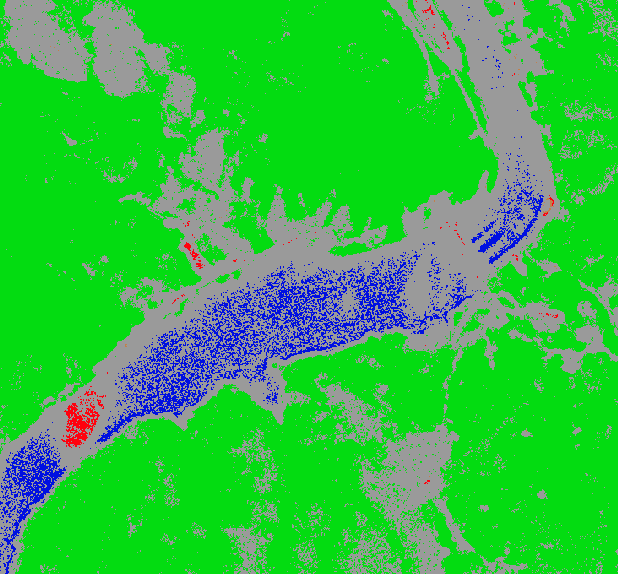
\includegraphics[width=0.45\linewidth]{drina-classification-no-pca}}
	\hspace{5pt}
	\subcaptionbox{A PCA-val betanított modell címkézése a Drinán}{
		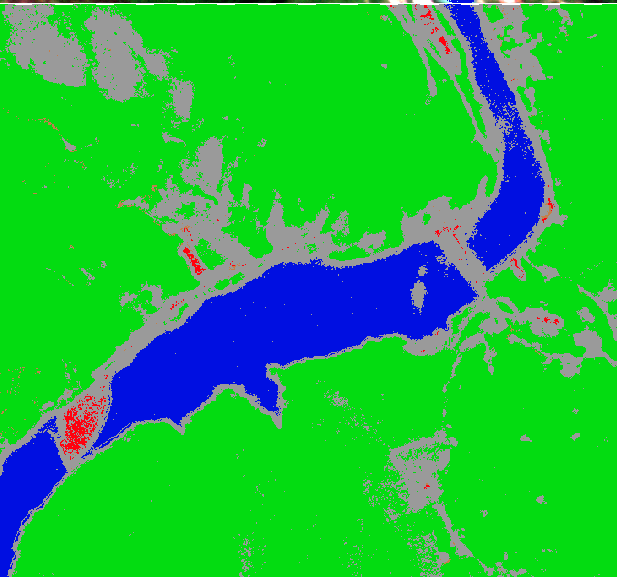
\includegraphics[width=0.45\linewidth]{drina-classification-with-pca}}
	\caption{A főkomponens analízissel betanított modell osztályozásának össszehasonlítása a PCA nélkül betanított modellel. Felvétel dátuma: 2023.05.21.}
	\label{fig:classification-pca-vs-no-pca}
\end{figure}

\section{Vízmaszkolás}
\todo[inline,color=blue!50]{A vízmaszkolásnak van egy műveleti költsége, így csak akkor fog megtérülni a használata, ha akkora területeket lehet kivágni vele, hogy jelentősen spórolunk azon, hogy azokon a területeken nem kell már hulladékot keresni. Emellett a víztől távoli \textit{false positive} detektálások számát is tudja növelni.\\
Tamás töltött le egy nagyobb területet, talán ezt:\\
https://gis.inf.elte.hu:9000/ws-waste-detection/satellite\_images/manual/planetscope/Tisza-Szabolcs\\
Ezen kiértékelve milyen futási idő jön ki? Ha ott sem jó, akkor a hangsúlyt a false positive-ok csökkentésére helyezném, nem a teljesítményre.\\
Röviden érdemes a vízmaszkolásról írni szerintem, ha más nem, akkor a future work-ben.\\
Tamás munkáját nehéz hivatkozni, mivel nem adta / adja le ebben a félévben a diplomamunkáját. Ezen a ponton elég lesz annyi, hogy a vízmaszkolást nem te implementáltad, hanem a labor egy másik résztvevője. \\
Botond: Igen, sajnos azon a felvételen értem el a rosszabb futási időt, amit linkeltél. Átfogalmaztam, a hangsújt az esetleges hamis riasztások csökkentésére fektettem.}

A kutatásunk hosszútávú célja a folyók közelében található hulladékkal szennyezett területeknek a detektálása, így a folyóktól távolabbi területeket érdemes kivágni a fölösleges riasztások elkerülésének érdekében. 
Ehhez használtam egy vízmaszkolási algoritmust, amit a laboron belül elkészített az egyik kollégám, és megvizsgáltam, hogy hogyan teljesít az új modell egy vízmaszk mellett. A \ref{fig:river-mask-performance} ábrán látható az, hogy a modell a folyótól távoli területeket nem osztályozza, így automatikusan a folyótól igen távol levő riasztások kizárásra kerülnek. Természetesen ez paraméterezhető, így ha mégis a Drina melletti hulladéklerakót is szeretnénk vizsgálni, akkor a vízmaszknak egy nagyobb távolságot be lehet állítani.

\begin{figure}[H]
	\centering
  \subcaptionbox{A Drina műholdfelvétele.}{
		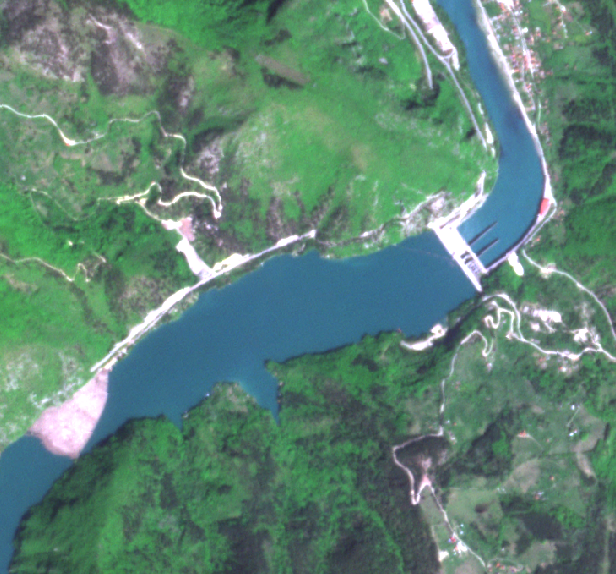
\includegraphics[width=0.45\linewidth]{drina-20230507}}
	\hspace{5pt}
	\subcaptionbox{A vízmaszk nélküli osztályozás.}{
		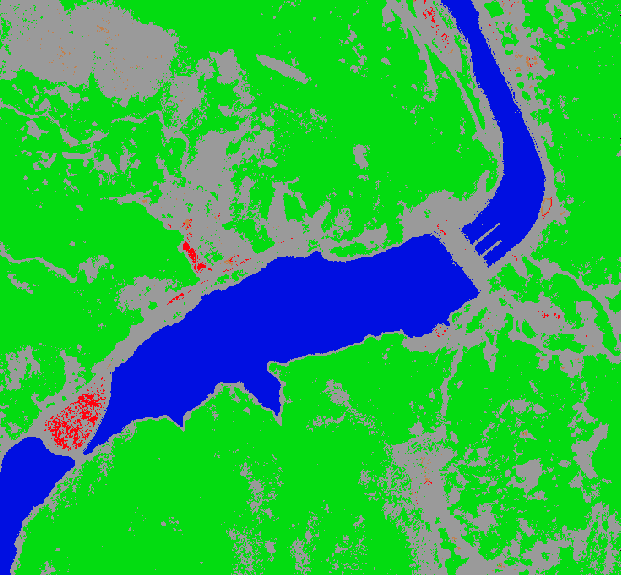
\includegraphics[width=0.45\linewidth]{drina-new-20230507}}
	\hspace{5pt}
	\subcaptionbox{A vízmaszkkal történő osztályozás.}{
		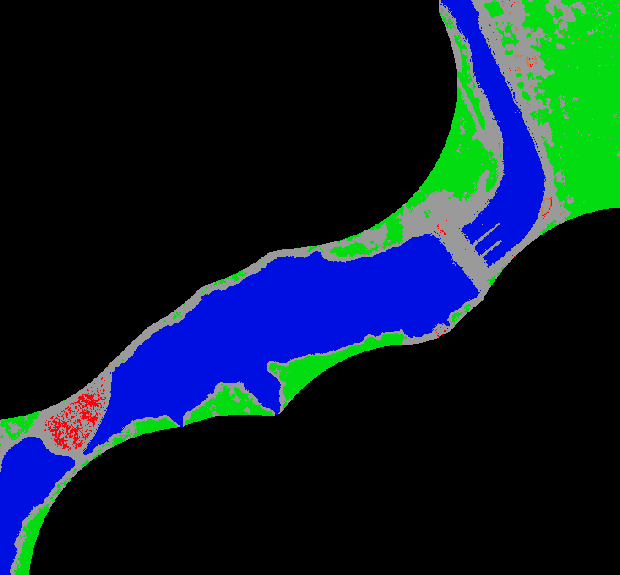
\includegraphics[width=0.45\linewidth]{drina-river-mask-20230507}}
	\caption{A vízmaszkolt osztályozás összehasonlítása a vízmaszk nélküli osztályozással. A Drina melletti hulladéklerakó kizárásra kerül. Felvétel dátuma: 2023.05.07.}
	\label{fig:river-mask-performance}
\end{figure}

\section{Nyári adatokon betanított modell teljesítménye}
\label{ch:summer-winter-models}

A nyári adatokon tanított modellnél javulásra lehet számítani az eredményekben, tekintve arra, hogy ez a modell erre az évszakra specializálódik. A \ref{tab:summer-winter-split} táblázatból látható, hogy a külön nyári felvételeken tanított modell picivel kevesebb false-positive-ot tartalmaz az általánosan betanított modellnél a nyári felvételeken. A \ref{fig:summer-vs-new} ábrából látható, hogy a nyári modell egy picivel jobban teljesít, mint az általános modell. Természetesen ebbe az irányba haladni azt az implikációt vonja maga után, hogy két modellt kell karbantartani egy modell helyett. Ugyanakkor a téli modell validálása külön kihívást jelent tekintve arra, hogy téli időszakban sokszor homályosak a felvételek a magasabb csapadékszint, és felhősebb viszonyok miatt, emiatt szabad szemmel nehezebb ellenőrizni a modell teljesítményét. Ennek fényében egy további lépése lehet a kutatásnak, hogy akár személyesen, akár magas felbontású drónfelvételek segítségével a téli felvételeket külön leellenőrizzük. 

\begin{table}[H]
	\centering
	\begin{tabular}{ | p{0.33\textwidth} | p{0.33\textwidth} | }
		\hline
		\textbf{Mérés azonosító} & \textbf{Nyári modell átlagai (\%)} \\
		\hline \hline
		\emph{Comission Rate} & 26.1 \\
		\hline
		\emph{Omission Rate} & 71.27  \\
		\hline
		\emph{Match Rate} & 28.05  \\
		\hline
        \emph{Extraction Rate} & 39.63 \\
		\hline
	\end{tabular}
	\caption{A nyári időszakra tanított modell átlagai}
	\label{tab:summer-winter-split}
\end{table}

\begin{figure}[H]
	\centering
  \subcaptionbox{A teszthalmaz kézi annotációja}{
		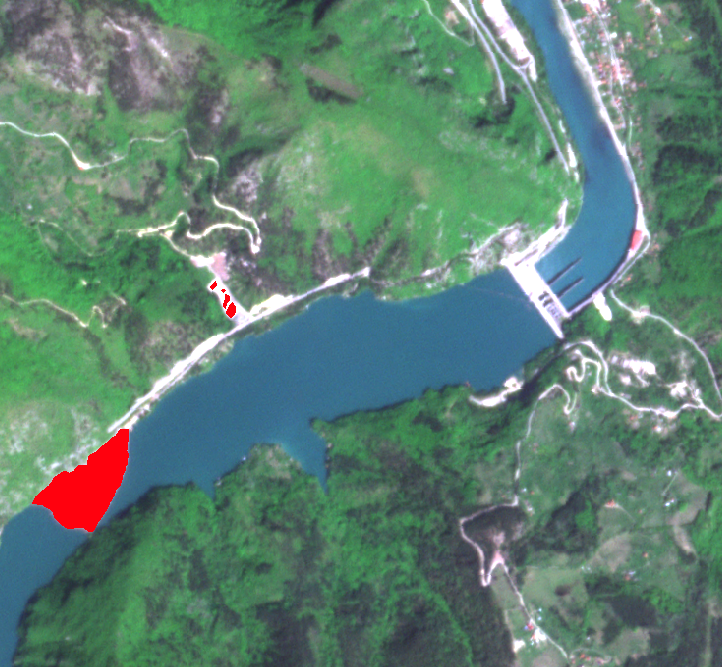
\includegraphics[width=0.45\linewidth]{drina-test}}
	\hspace{5pt}
	\subcaptionbox{A teszthalmaz annotációja az új modellel}{
		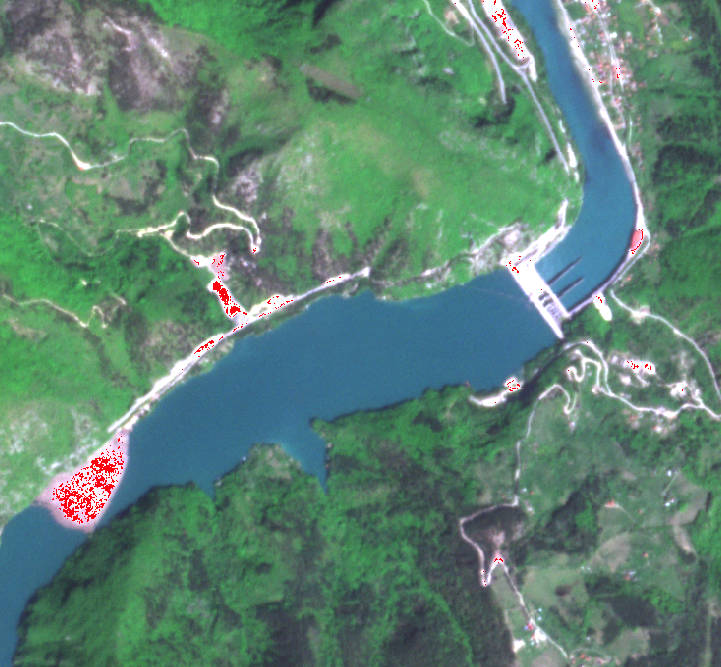
\includegraphics[width=0.45\linewidth]{drina-new}}
	\hspace{5pt}
	\subcaptionbox{A teszthalmaz annotációja a nyári modellel}{
		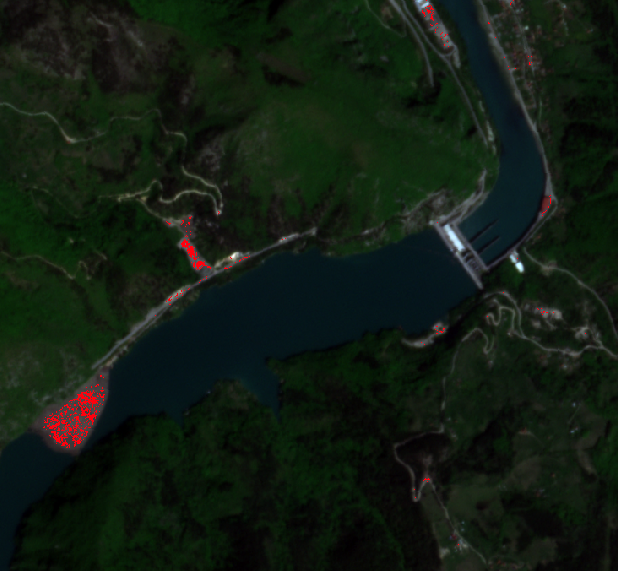
\includegraphics[width=0.45\linewidth]{drina-summer}}
	\caption{Az új modell összehasonlítása a nyári modellel az egyik Drinai teszt felvételen. Felvétel dátuma: 2023.05.07.}
	\label{fig:summer-vs-new}
\end{figure}

\section{Normalizálás tesztelése}
\label{ch:normalization-test} 

A normalizálásnak az volt a motivációja, hogy azokat a felvételeket, amik spektrális értékeikben lényeges eltéréseket tartalmaznak a többi felvételhez képest, tudjam értelmezhetővé tenni a modell számára. Teszteléshez kiválasztottam egy nyári Drinai felvételt, amin az új modell rosszul teljesített, és összehasonlítottam a normalizált képeken betanított modell eredményeivel. A \ref{fig:normal-vs-normalized-vs-old} ábrán látható, hogy a régi modell ezen a felvételen detektálta a hulladékszigetet, de vele együtt detektált nagyon sok false-positive-et is. Az új, normalizálás nélküli modell nagyon kevés hulladékot detektált, míg a normalizált modell ugyancsak sok false-positive-ot detektált. Habár első körben a normalizálással nem a várt eredményeket értem el, egy további kutatási irány lehet ennek a továbbvizsgálása, esetleg más referenciafelvételek megválasztása.

\begin{figure}[H]
	\centering
  \subcaptionbox{A régi modell teljesítménye}{
		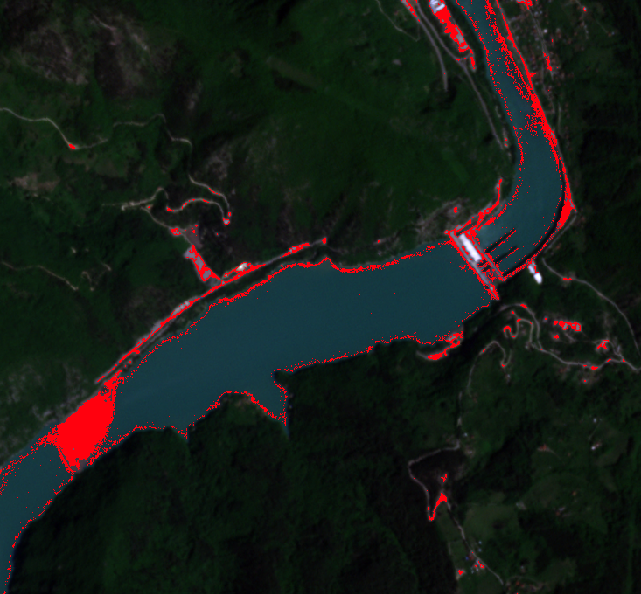
\includegraphics[width=0.45\linewidth]{drina-old-model-20230524}}
	\hspace{5pt}
	\subcaptionbox{Az új, normalizáció nélküli modell teljesítménye}{
		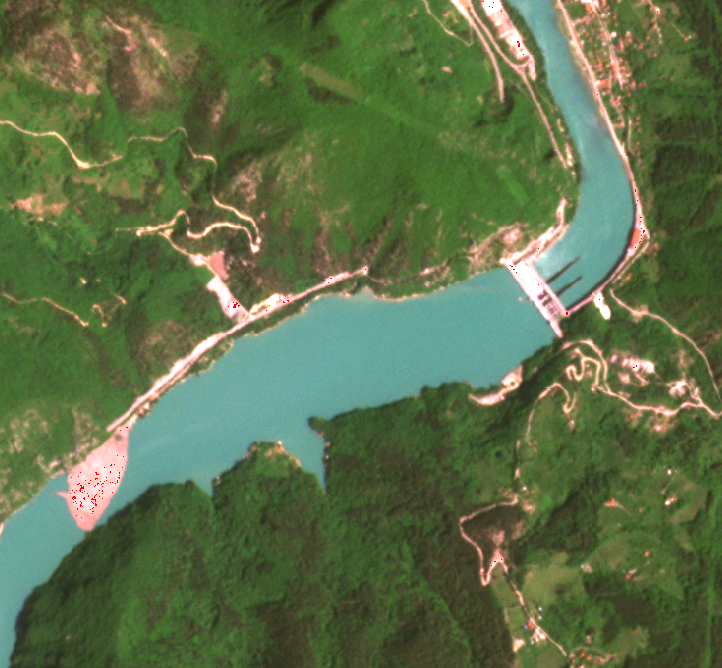
\includegraphics[width=0.45\linewidth]{drina-with-extra-unknowns-model-20230524}}
	\hspace{5pt}
	\subcaptionbox{Az új, normalizációval tanított modell teljesítménye}{
		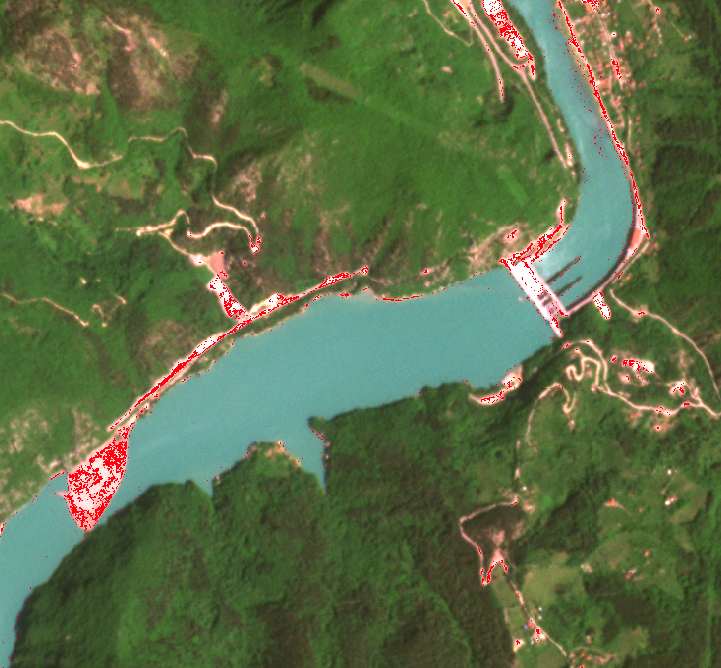
\includegraphics[width=0.45\linewidth]{drina-reference-model-20230524}}
	\caption{A régi, a normalizáció nélkül tanított és a normalizációval tanított modell összehasonlítása a Drinán. Felvétel dátuma: 2023.05.24.}
	\label{fig:normal-vs-normalized-vs-old}
\end{figure}


\section{Empirikus validáció}
\label{ch:empirical-validation}
Az empirikus validáció alá esnek a téli drinai és nyári kiskörei felvételek. Ennek az az oka, hogy a téli drinai felvételek közül kihívás volt megfelelő minőségű felvételt találni numerikus validációra, míg a 2023-as kiskörei adathalmaz tanításra volt használva, így a 2024-es adathalmazból való felvételek is alkalmatlannak bizonyultak numerikus validációra. 

A \ref{fig:drina-winter-all-models} ábrából látható, hogy a téli felvételen árnyék takarja a hulladéksziget felét. Itt látszik, hogy a modellek számára nehézséget jelent az árnyék alatt levő hulladéksziget detektálása. Az egyetlen modell, aki képes volt detektálni az árnyék alatti szigetet, az a régi modell volt, de cserében nagyon sok false-positive-ot termelt a többi modellhez képest. Így, a kutatás jelenlegi állapotában a téli hulladékdetektálás jelenti az egyik nagy kihívást.

A \ref{fig:kiskore-all-models} ábrán egy kiskörei felvételen hasonlítottam össze az összes modellt. A három legjobban teljesítő modell az új modell, a nyári adatokon betanított új modell, illetve a főkomponens analízissel betanított modell. Míg a nyári adatokon tanított modell közel teljesített az új modellhez képest, a főkomponens analízissel betanított modell több területet hulladékosnak jelölt a szeméttorlaszon, de cserében intenzívebbek is voltak a false-positive értékek.

\begin{figure}[H]
	\centering
  \subcaptionbox{A teszthalmaz kézi annotációja}{
		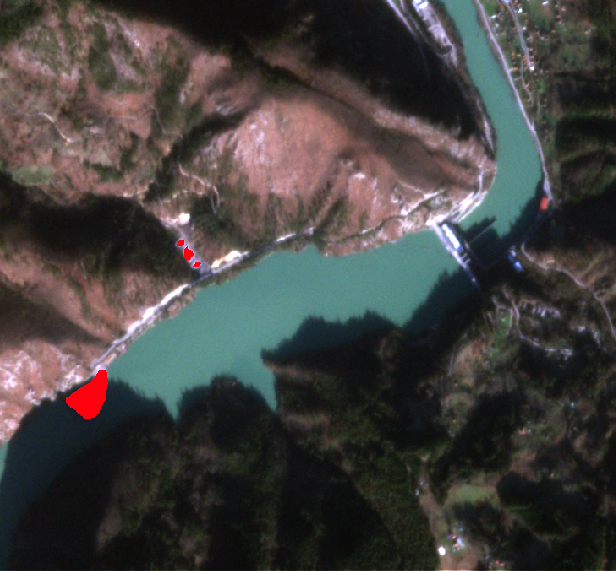
\includegraphics[width=0.45\linewidth]{drina-test-20231217}}
	\hspace{5pt}
	\subcaptionbox{A teszthalmaz annotációja a régi modellel}{
		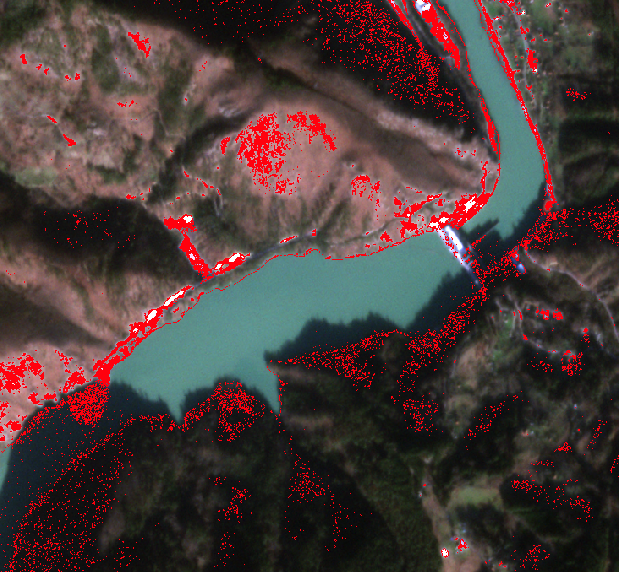
\includegraphics[width=0.45\linewidth]{drina-old-20231217}}
	\hspace{5pt}
	\subcaptionbox{A teszthalmaz annotációja az új modellel}{
		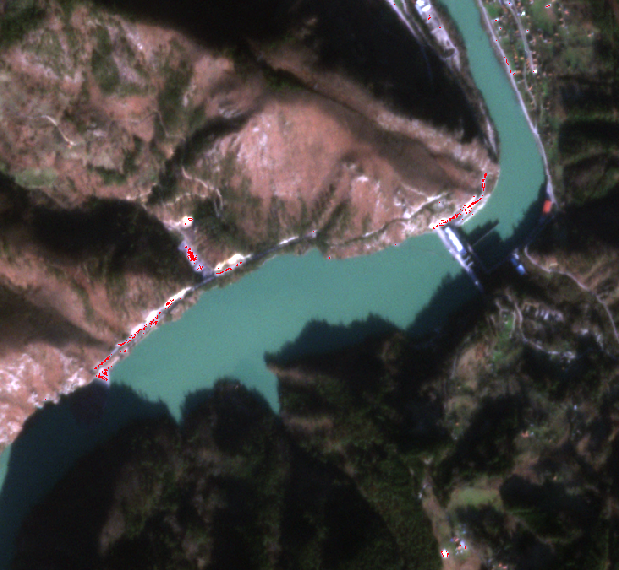
\includegraphics[width=0.45\linewidth]{drina-new-20231217}}
	\hspace{5pt}
	\subcaptionbox{A teszthalmaz annotációja a téli modellel}{
		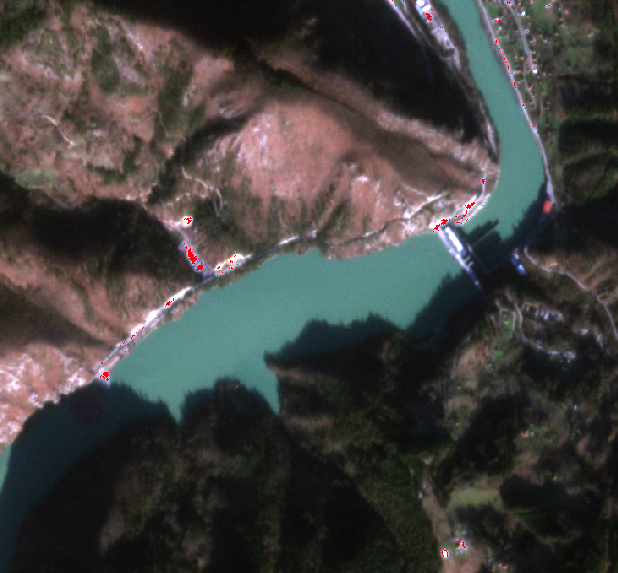
\includegraphics[width=0.45\linewidth]{drina-winter-20231217}}
	\hspace{5pt}
	\subcaptionbox{A teszthalmaz annotációja a normalizált modellel}{
		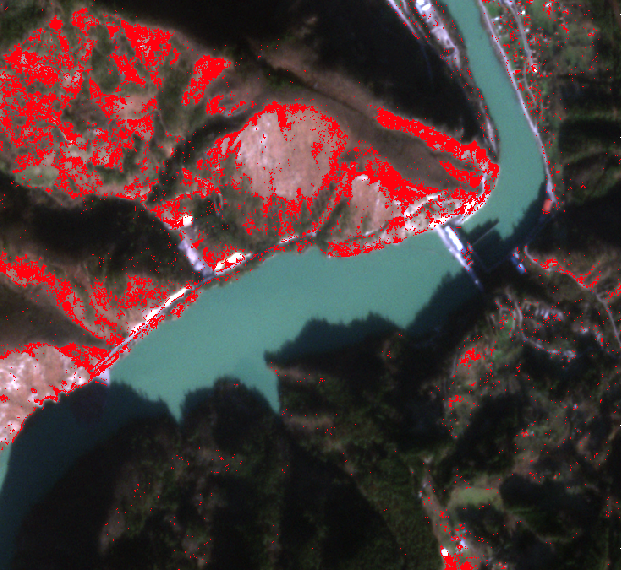
\includegraphics[width=0.45\linewidth]{drina-reference-20231217}}
	\hspace{5pt}
	\subcaptionbox{A teszthalmaz annotációja a PCA-val tanított modellel}{
		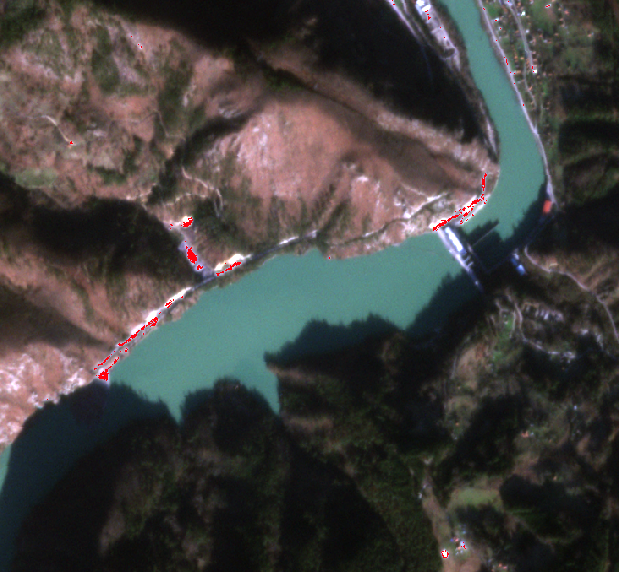
\includegraphics[width=0.45\linewidth]{drina-pca-20231217}}
	\caption{Az összes modell összehasonlítása az egyik téli drinai teszt felvételen. Felvétel dátuma: 2023.12.17.}
	\label{fig:drina-winter-all-models}
\end{figure}

\begin{figure}[H]
	\centering
  \subcaptionbox{A teszthalmaz kézi annotációja}{
		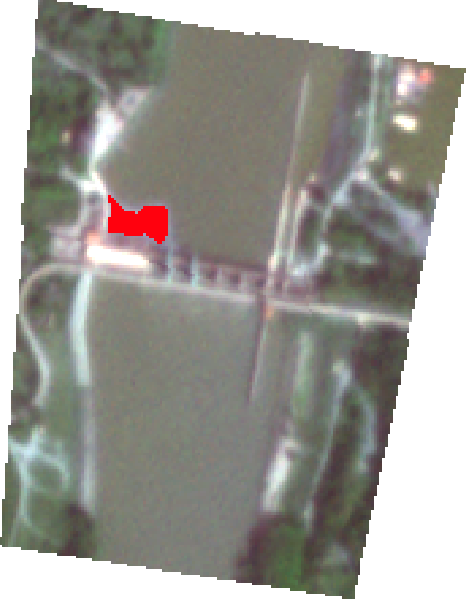
\includegraphics[width=0.30\linewidth]{kiskore-test-20240412}}
	\hspace{5pt}
	\subcaptionbox{A teszthalmaz annotációja a régi modellel}{
		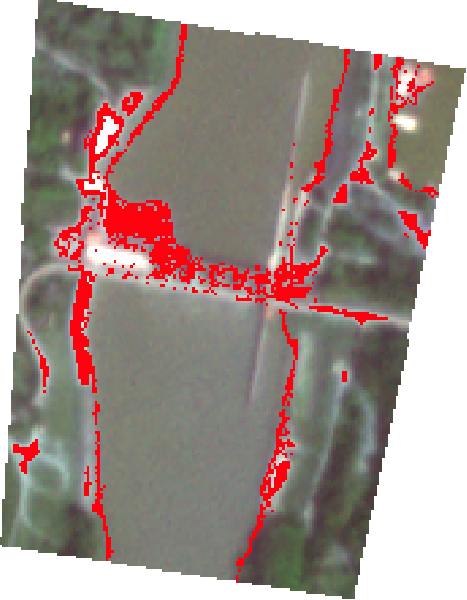
\includegraphics[width=0.30\linewidth]{kiskore-old-20240412}}
	\hspace{5pt}
	\subcaptionbox{A teszthalmaz annotációja az új modellel}{
		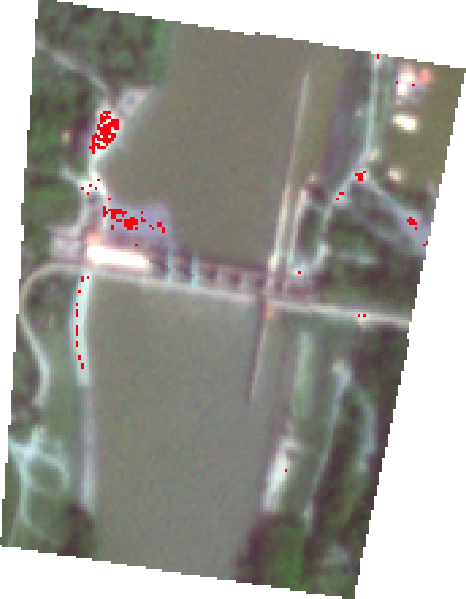
\includegraphics[width=0.30\linewidth]{kiskore-new-20240412}}
	\hspace{5pt}
	\subcaptionbox{A teszthalmaz annotációja a nyári modellel}{
		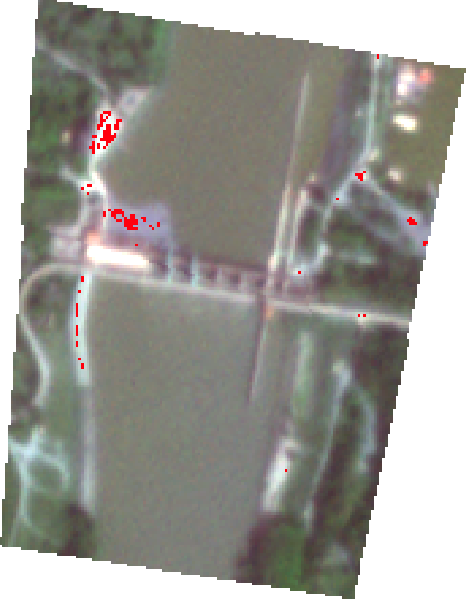
\includegraphics[width=0.30\linewidth]{kiskore-summer-20240412}}
	\hspace{5pt}
	\subcaptionbox{A teszthalmaz annotációja a normalizált modellel}{
		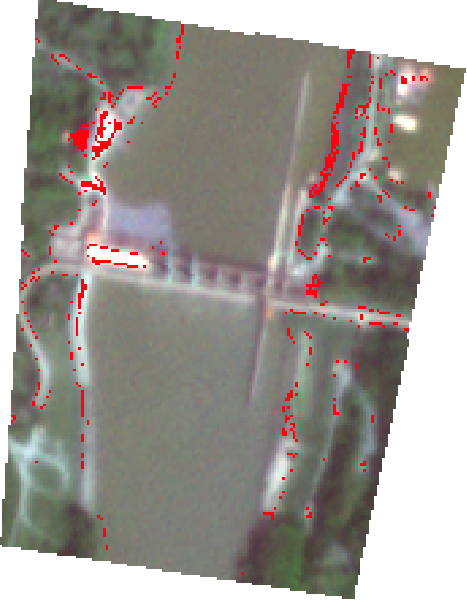
\includegraphics[width=0.30\linewidth]{kiskore-reference-20240412}}
	\hspace{5pt}
	\subcaptionbox{A teszthalmaz annotációja a PCA-val tanított modellel}{
		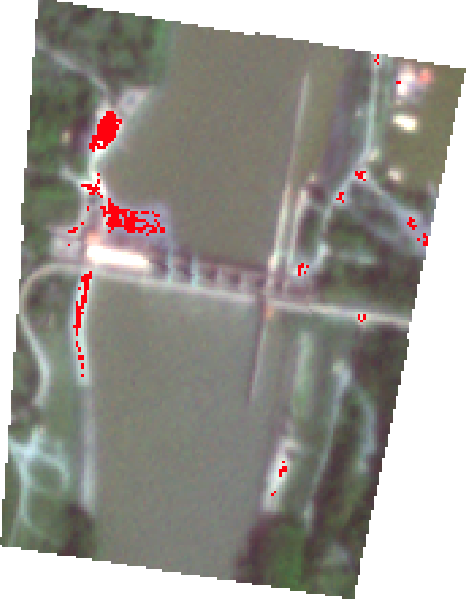
\includegraphics[width=0.30\linewidth]{kiskore-pca-20240412}}
	\caption{Az összes modell összehasonlítása az egyik kiskörei teszt felvételen. Felvétel dátuma: 2024.04.12.}
	\label{fig:kiskore-all-models}
\end{figure}

\chapter{Megvalósítás és alkalmazás}
\label{ch:impl}

\subsection{A meglevő alkalmazások bővítése}
\label{ch:application-improvement}

\subsubsection {Az asztali alkalmazás bővítése}

A meglevő asztali alkalmazás alkalmas volt a tanítóadatok hatékony előállítására, de utólag nem lehetett visszanézni, hogy adott műholdfelvételhez milyen tanítóadatok tartoznak, illetve azt sem, hogy az adott tanítóadat hol volt mintavételezve. Az alkalmazás eredetileg egy CSV fájlba eltárolta az összes pixel spektrális értékeit és indexeit, és ezt lehetett használni tanításra. Ennek az volt a hátránya, hogy nehéz volt áttekinteni illetve kiegészíteni az adatokat. Ezért az asztali alkalmazást kiegészítettem ezzel a funkcionalitással, a tanítóadatok előállítása elmentésekor az alkalmazás létrehoz egy külön raszteres réteget is külön minden műholdfelvételhez, melyen látható, hogy mely területek voltak hozzáadva a tanítóadatok közé, így tetszőleges módon előállítható/ellenőrizhető a tanítóhalmaz.

\subsubsection {A szerveralkalmazás bővítése}

A szerveralkalmazás és webalkalmazás is bővítésre került: a szerveralkalmazás mostmár több modellt is le tud futtatni a letöltött műholdfelvételeken és ezeket külön tárolja. A webalkalmazás mostmár képes letölteni külön ezeket az eredményeket és több hulladékmaszkoló módszer eredményét is meg tudja jeleníteni, ennek köszönhetően ezeket egymással össze lehet könnyen hasonlítani valós tesztadatokon. 

\subsection{A Tiszta-Tisza alkalmazás}

A Tiszta-Tisza webalkalmazás \todo{melyik link kerüljön ide?} a PET Kupa által használt webalkalmazás, melynek az a célja, hogy egy olyan felületet biztosítson, ahol meglehet tekinteni a jelenleg ismert folyómentén található hulladéklerakókat, illetve akár a regisztrált felhasználók is be tudnak jelenteni ilyet. A PET Kupa megbízta az egyetemet azzal a feladattal, hogy ezt továbfejlessze, és a feladatok közé tartozott az is, hogy a Random Forest modell eredményeit integráljuk ebbe az alkalmazásba. Ezt a feladatot én vállaltam el.

Tekintve arra, hogy a Tiszta-Tisza térképén pontok vannak megjelenítve, a modell által detektált területeket is pontokkal jelöljük. Ehhez egy nagyobb terület közepére helyezünk el egy pontot. Előfordulhat olyan is, hogy a modell olyan képeket klasszifikál, melyek el vannak torzítva (például magas páratartalom miatt). Ilyenkor a false-positive-ok aránya lényegesen megnő. Ennek korrigálására a Tiszta-Tisza alkalmazásban a legutolsó három detektálást (legfeljebb 1 hónap különbséggel) veszem figyelembe és két kép közös metszetével döntöm el, hogy milyen területek kerülnek fel a térképre. A lépéseket a \ref{ch:intersection} fejezetben részletezem.

\subsection{Közös metszet}
\label{ch:intersection}

A már meglevő szervertől poligonok formájában, GeoJSON-ben \cite{rfc7946} lehet lekérni az adott napon detektált hulladékos területeket. így érdemes poligonok metszetében kigondolni a többségi szavazást. Jelöljük BUF(P,n)-vel egy multipoligon pufferét, ahol $$P \in \mathbb{P}$$ egy multipoligon, és n egy egész szám. Ekkor a többségi szavazást három képre a \ref{eq:voting} \todo{hasonló képleteket mások is ismernek fórumokban, de hivatalos forrással nem találkoztam} képlet szerint lehet alkalmazni. Ezután az elég nagy poligonok egy-egy belső pontját megválasztva megtudjuk jelölni a hulladéklerakókat.

\begin{equation}\label{eq:voting}
    Eredm\acute{e}ny \ multipoligon = \bigcup_{P_1 \in \mathbb{P}} \bigcup_{P_2 \in \mathbb{P}} BUF(BUF(P_1,n) \cap BUF(P_2,n),-n)
\end{equation}
\cleardoublepage

\chapter{Összefoglalás és eredmények}
\label{ch:sum}

\section{A kutatás során elért eredmények}

A dolgozatomban megvizsgáltam több módszert, amivel a korábbi modellben levő kihívásokat korrigáltam multispektrális Planetscope felvételeken. Előállítottam egy tanító adathalmazt, ami segítségével meg lehet vizsgálni több gépi tanulási módszert, illetve ki lehet próbálni több képfeldolgozási módszert. Megmutattam, hogy egy nagyobb tanító halmaz segítségével alacsonyabb false-positive arányokkal tudja a Random Forest modell detektálni a hulladékkal szennyezett területeket a teszthalmazban. Kiegészítettem az ELTE IK Térinformatikai laborban használt eszközöket arra, hogy hatékonyabban lehessen előkészíteni és megvizsgálni a különböző hulladékdetektálási módszereket. Megvizsgáltam a főkomponens analízis hatását a Random Forestre, és arra a következtetésre jutottam, hogy a modell láthatóan jobban kezelte PCA-val a többdimenziós felvételekben levő zajt, mint a PCA nélküli modell. Továbbá megnéztem, hogy miként teljesít a modell képnormalizálás, illetve vízmaszkolás mellett. Az utóbbi két módszert a laborban kutatják és fejlesztik a kollégáim. Bemutattam a módszer használhatóságát azzal, hogy a Tiszta-Tisza webalkalmazásába integráltam a Random Forest modell eredményeit, egyszerű poligonműveletek segítségével.

\section{A kutatás kihívásai}

A kutatás talán legnagyobb kihívása a tanító adatok megfelelő előállítása és a modellek validációja. A \ref{ch:waste-detection-methods} fejezetben bemutatott hulladékdetektálási módszerekben gyakori módszer volt egy magas felbontású műholdfelvétel használata validációra, vagy nagyon magas felbontású drónfelvételek használata a vizsgált területeken. A modell vizsgálata téli felvételeken is egy kihívás tekintve arra, hogy télen ritkábbak a megfelelő időjárás körülmények a nyári időszakokhoz képest. 

\section{További lépések}

A továbbiakban érdemes megvizsgálni akár személyesen, akár magas felbontású felvételekből a hulladékkal szennyezett területeket pontosabb validáció érdekében. Az adat-normalizálási módszereket is érdemes továbbvizsgálni, tekintve arra, hogy gyakori a zaj a műholdfelvételekben, így ilyen módszerek lényegesen növelhetik a modell megbízhatóságát. További lépésként javasolt akár más gépi tanulási módszereket is kipróbálni, illetve klasszikusabb térinformatikai eszközökkel is megközelíteni a hulladékdetektálás problémáját. Gépi tanulási irány esetén érdemes egy sokkal nagyobb adathalmazt előállítani, pontosabb adatvizsgálat mellett, így a modellek jobban tudják majd általánosítani az adatokat hulladékdetektálás céljából.

\cleardoublepage

% Acknowledgements (optional) - in case your thesis received funding or would like to express special thanks to someone
\chapter*{\acklabel}
\addcontentsline{toc}{chapter}{\acklabel}
Köszönetet szeretnék mondani az ELTE Informatikai Karának a TDK ösztöndíj biztosításáért, illetve a PET Kupának a projekt szakmai támogatásáért. Külön köszönet jár a témavezetőmnek, Cserép Máténak, aki szakmailag eligazított a kutatásomban. Köszönetet szeretnék mondani az ELTE IK Térinformatika Laborban levő munkatársaimnak, akikkel együtt dolgoztunk, és akik nélkül nem tartana itt a kutatás. Köszönetet szeretnék mondani a Planet Labs-nak is, akik kutatási célból ingyenesen biztosítottak műholdfelvételeket a labor számára.


% Appendices (optional) - useful for detailed information in long tables, many and/or large figures, etc.
% \appendix
% \chapter{Szimulációs eredmények}
\label{appx:simulation}

Lorem ipsum dolor sit amet, consectetur adipiscing elit. Pellentesque facilisis in nibh auctor molestie. Donec porta tortor mauris. Cras in lacus in purus ultricies blandit. Proin dolor erat, pulvinar posuere orci ac, eleifend ultrices libero. Donec elementum et elit a ullamcorper. Nunc tincidunt, lorem et consectetur tincidunt, ante sapien scelerisque neque, eu bibendum felis augue non est. Maecenas nibh arcu, ultrices et libero id, egestas tempus mauris. Etiam iaculis dui nec augue venenatis, fermentum posuere justo congue. Nullam sit amet porttitor sem, at porttitor augue. Proin bibendum justo at ornare efficitur. Donec tempor turpis ligula, vitae viverra felis finibus eu. Curabitur sed libero ac urna condimentum gravida. Donec tincidunt neque sit amet neque luctus auctor vel eget tortor. Integer dignissim, urna ut lobortis volutpat, justo nunc convallis diam, sit amet vulputate erat eros eu velit. Mauris porttitor dictum ante, commodo facilisis ex suscipit sed.

Sed egestas dapibus nisl, vitae fringilla justo. Donec eget condimentum lectus, molestie mattis nunc. Nulla ac faucibus dui. Nullam a congue erat. Ut accumsan sed sapien quis porttitor. Ut pellentesque, est ac posuere pulvinar, tortor mauris fermentum nulla, sit amet fringilla sapien sapien quis velit. Integer accumsan placerat lorem, eu aliquam urna consectetur eget. In ligula orci, dignissim sed consequat ac, porta at metus. Phasellus ipsum tellus, molestie ut lacus tempus, rutrum convallis elit. Suspendisse arcu orci, luctus vitae ultricies quis, bibendum sed elit. Vivamus at sem maximus leo placerat gravida semper vel mi. Etiam hendrerit sed massa ut lacinia. Morbi varius libero odio, sit amet auctor nunc interdum sit amet.

Aenean non mauris accumsan, rutrum nisi non, porttitor enim. Maecenas vel tortor ex. Proin vulputate tellus luctus egestas fermentum. In nec lobortis risus, sit amet tincidunt purus. Nam id turpis venenatis, vehicula nisl sed, ultricies nibh. Suspendisse in libero nec nisi tempor vestibulum. Integer eu dui congue enim venenatis lobortis. Donec sed elementum nunc. Nulla facilisi. Maecenas cursus id lorem et finibus. Sed fermentum molestie erat, nec tempor lorem facilisis cursus. In vel nulla id orci fringilla facilisis. Cras non bibendum odio, ac vestibulum ex. Donec turpis urna, tincidunt ut mi eu, finibus facilisis lorem. Praesent posuere nisl nec dui accumsan, sed interdum odio malesuada.
% \cleardoublepage

% Bibliography (mandatory)
\phantomsection
\addcontentsline{toc}{chapter}{\biblabel}
\printbibliography[title=\biblabel]
\cleardoublepage

% List of figures (optional) - useful over 3-5 figures
\phantomsection
\addcontentsline{toc}{chapter}{\lstfigurelabel}
\listoffigures
\cleardoublepage

% List of tables (optional) - useful over 3-5 tables
\phantomsection
\addcontentsline{toc}{chapter}{\lsttablelabel}
\listoftables
\cleardoublepage

% List of algorithms
% \phantomsection
% \addcontentsline{toc}{chapter}{\lstalgorithmlabel}
% \listofalgorithms
% \cleardoublepage

% List of codes (optional) - useful over 3-5 code samples
% \phantomsection
% \addcontentsline{toc}{chapter}{\lstcodelabel}
% \lstlistoflistings
% \cleardoublepage

% List of symbols (optional)
%\printnomenclature

\end{document}
